%%%%%%%%%%%%%%%%%%%%%%
\documentclass{singlecol-new}
%%%%%%%%%%%%%%%%%%%%%%

\usepackage{natbib,stfloats}
\usepackage{mathrsfs}

\usepackage{graphicx}
%\usepackage[T1]{fontenc}
\usepackage{amsmath,amssymb}
\usepackage{float} 
\usepackage{enumerate}
\usepackage{algorithm,algorithmic}
 \usepackage{caption}
 \usepackage{url}
 
 \usepackage{mathtools}

\def\newblock{\hskip .11em plus .33em minus .07em}

\theoremstyle{TH}{
\newtheorem{lemma}{Lemma}
\newtheorem{theorem}[lemma]{Theorem}
\newtheorem{corrolary}[lemma]{Corrolary}
\newtheorem{conjecture}[lemma]{Conjecture}
\newtheorem{proposition}[lemma]{Proposition}
\newtheorem{claim}[lemma]{Claim}
\newtheorem{stheorem}[lemma]{Wrong Theorem}
%\newtheorem{algorithm}{Algorithm}
}

\theoremstyle{THrm}{
\newtheorem{definition}{Definition}[section]
\newtheorem{question}{Question}[section]
\newtheorem{remark}{Remark}
\newtheorem{scheme}{Scheme}
}

\theoremstyle{THhit}{
\newtheorem{case}{Case}[section]
}

\makeatletter
\def\theequation{\arabic{equation}}

\JOURNALNAME{\TEN{\it I. J. of Industrial and Systems Engineering, Vol. \theVOL, No. \theISSUE, \thePUBYEAR}\hfill\thepage}%

\def\BottomCatch{%
\vskip -10pt
\thispagestyle{empty}%
\begin{table}[b]%
\NINE\begin{tabular*}{\textwidth}{@{\extracolsep{\fill}}lcr@{}}%
\\[-12pt]
Copyright \copyright\ 20xx Inderscience Enterprises Ltd. & &%
\end{tabular*}%
\vskip -30pt%
%%\vskip -35pt%
\end{table}%
} \makeatother

\DeclarePairedDelimiter{\ceil}{\lceil}{\rceil}		
\DeclarePairedDelimiter{\floor}{\lfloor}{\rfloor}

%%%%%%%%%%%%%%%%%
\begin{document}%
%%%%%%%%%%%%%%%%%

\setcounter{page}{1}

\LRH{G. Clímaco et~al.}

\RRH{New approaches for the  PCCTP}

\VOL{x}

\ISSUE{x}

\PUBYEAR{201X}

\BottomCatch

\CLline

\subtitle{}

\title{New approaches for the  Prize-Collecting Covering Tour problem}

%
\authorA{Glaubos Clímaco*}
% %
\affA{Departamento de informática,\\ Universidade Federal do Maranhão,\\ São Luís, Brazil \\
E-mail: francisco.glaubos@ufma.br\\
*Corresponding author}
% %
% %
\authorB{Luidi Simonetti}
\affB{Programa de Engenharia de Sistemas e Computação,\\ Universidade Federal do Rio de Janeiro,\\ Rio de Janeiro, Brazil \\
E-mail: luidi@cos.ufrj.br}

\authorC{Isabel Rosseti}
\affC{Instituto de Computação, \\ Universidade Federal Fluminense,\\ Niterói, Brazil\\
E-mail: rosseti@ic.uff.br}

\authorD{Pedro Henrique González}
\affD{Departamento de Ciência da Computação,\\Centro Federal de Educação Tecnológica Celso Suckow da Foseca,\\
Rio de Janeiro, Brazil\\
E-mail: pegonzalez@eic.cefet-rj.br}

%
%\authorA{Fusheng Wang\footnote{Work done while working at Siemens Corporate Research.} }
%
%\affA{Department of Biomedical Informatics, Emory University
%\newline
%36 Eagle Row, Ste 589, Atlanta, GA 30322, USA}
%
%
%
%\authorB{\footnotesize Cristobal Vergara-Niedermayr\footnote{Work done while working at Siemens Corporate Research.}}
%\affB{Oracle \newline
 %New Jersey, USA}
%
%
% \authorC{Peiya Liu}
% \affC{Department of Integrated Data Systems, Siemens Corporate
% Research \newline 755 College Road East, Princeton 08540, USA}

\begin{abstract}
In this paper, we consider the   Prize-Collecting Covering Tour problem (PCCTP), which intends to find a minimum cost tour for travelling teams that grant assistance to people located far from urban centers. We develop a branch-and-cut algorithm, some valid inequalities, and a new set of reduction rules as exact approaches. We also present a hybrid heuristic that combines a state-of-the-art heuristic for the PCCTP  with  integer programming techniques. Computational experiments showed that the exact approaches  found several new optimal solutions while reducing CPU time, and the hybrid heuristic was able to match or improve the solution quality for many instances, along with a significant reduction of running time.
\end{abstract}

\KEYWORD{PCCTP; GRASP; RVND; hybrid heuristic; reduction rules}

% \REF{to this paper should be made as follows: Rodr\'{\i}guez
% Bol\'{\i}var, M.P. and Sen\'{e}s Garc\'{\i}a, B. (201X) `The
% corporate environmental disclosures on the internet: the case of
% IBEX 35 Spanish companies', {\it International Journal of Metadata,
% Semantics and Ontologies}, Vol. x, No. x, pp.xxx\textendash xxx.}

\begin{bio}
Glaubos Clímaco received his BSc in Computer Science
from the Universidade Federal do Tocantins in 2013, Master’s in Computing
from the Universidade Federal Fluminense in 2015 and PhD in Systems and
Computer Engineering from the Universidade Federal do Rio de Janeiro in
2020. Currently, he is an Assistant Professor at the Federal University of
Maranhão. He has experience in computer science, with an emphasis on
operations research, working mainly on the following topics: heuristics, traffic
counting location problem, location of traffic counters, and brkga. \vs{8}

\noindent Luidi Simonetti graduated in Mechanical Engineering from the Federal University of Rio de Janeiro(2000), Master's in Systems and Computer Engineering from the Federal University of Rio de Janeiro(2003), Ph.D. in Systems and Computer Engineering from the Federal University of Rio de Janeiro(2008 ) and post-doctorate at the State University of Campinas(2010). He has experience in Computer Science, with an emphasis on Mathematical Programming. Mainly working on the following topics: Spanning Trees, combinatorial optimisation, branch-and-cut. \vs{8}

\noindent Isabel Rosseti has a degree in Computer Engineering from the Federal University of Espírito Santo (1995), a Master's in Informatics from the Pontifical Catholic University of Rio de Janeiro (1998) and a Ph.D. in Informatics from the Pontifical Catholic University of Rio de Janeiro (2003). She is currently an associate professor at the Universidade Federal Fluminense. She has experience in Computer Science and Combinatorial Optimisation, working mainly on the following topics: heuristics, hybridisation of heuristics with data mining and exact methods.

\noindent Pedro Henrique González graduated in Mathematics from the State University of Rio de Janeiro (2009). Master in Computer Science from the State University of Rio de Janeiro (2012). PhD in Computing from the Fluminense Federal University (2015) and in Informatique from the University of Avignon and Pays de Vaucluse in a co-tutorship scheme (2015). He conducted postdoctoral research at the Federal University of Rio de Janeiro with a focus on Combinatorial Optimisation (2016). EBTT Professor at the Federal Center for Technological Education of Rio de Janeiro (CEFET/RJ) since 2017, working in the Department of Informatics (DEPIN), in the Postgraduate Program in Computer Science (PPCIC), since 2019, and in the Program Postgraduate in Production and Systems Engineering (PPPRO), since 2021. Leader of the Combinatorial Optimisation and Applications research group (OCA/CNPq). He has interest and experience in the areas: Combinatorial Optimisation, Metaheuristics, Linear and Integer Programming, Hybrid Methods, Operations Research and Algorithm Design.

% Manuel Pedro Rodr\'iguez Bol\'ivar received his PhD in Accounting at
% the University of Granada. He is a Lecturer at the Department of
% Accounting and Finance, University of Granada. His research
% interests include issues related to conceptual frameworks of
% accounting, diffusion of financial information on Internet, Balanced
% Scorecard applications and environmental accounting. He is author of
% a great deal of research studies published at national and
% international journals, conference proceedings as well as book
% chapters, one of which has been edited by Kluwer Academic
% Publishers.\vs{9}

% \noindent Bel\'en Sen\'es Garc\'ia received her PhD in Accounting at
% the University of Granada. She is a Lecturer at the Department of
% Accounting and Finance, University of Granada. Her research
% interests are related to cultural, institutional and historic
% accounting and in environmental accounting. She has published
% research papers at national and international journals, conference
% proceedings as well as chapters of books.\vs{8}

% \noindent Both authors have published a book about environmental
% accounting edited by the Institute of Accounting and Auditing,
% Ministry of Economic Affairs, in Spain in October 2003.
\end{bio}


\maketitle

\section{Introduction}
\label{sec:intro}
%  \onehalfspacing
Although we live in an increasingly globalised world, there are still people living far away from the centers of big cities. Some types of services provided, such as legal services of justice, medical care, and social assistance are only available in large cities, which makes life difficult for people who live in more distant regions.

A simplistic solution would be to establish fixed units in each of these regions, but this is financially unfeasible, in addition to the fact that certain locations are inaccessible by land, which would make it difficult to maintain these facilities. One of the most adopted solutions in this case is the sending of itinerant teams, who make a route that covers all these locations that need assistance, passing and providing assistance in places at a maximum distance from where these people live, thus enabling them to be served.

An example of this scenario can be seen in the project \textit{Saúde Itinerante} carried out by the Health Department of the State of Pará (Brazil).  In this project, a vehicle adapted as a basic health unit carried out actions that covered six regions of Pará, benefiting the populations of 26 municipalities, with medical appointments in the areas of Internal Medicine, Paediatrics and Gynaecology, including scheduling appointments and specialised procedures, guidance nutritional, educational and preventive lectures on Oral Health with the delivery of oral hygiene kits, Women's Health and Men's Health, especially in the months dedicated to the prevention of cervical cancer, breast cancer and prostate cancer. Rapid tests for HIV, syphilis, hepatitis B and C, condom distribution, blood pressure measurement, blood glucose test, vaccines and the issuance of a national SUS card were also made available. In this context, the Covering Tour Problem (CTP) emerged. The CTP consists of determining a minimum length tour or Hamiltonian cycle on a subset of vertices such that every vertex to be covered is within a pre-specified distance from the cycle \citep{gendreau1997covering}.

In this paper, we  approach the Prize-Collecting Covering Tour problem (PCCTP) which can be considered as a variant of the CTP \citep{gendreau1997covering}. Since the CTP was proposed, several generalisations have emerged. Some of these generalisations consider several vehicles simultaneously  \citep{karimi2018capacitated, murakami2018iterative, margolis2021multi, karaouglan2018multi, glize2020exact, kammoun2020two}. Other variants address bi-objective models  that are directly related to the minimisation/maximisation of the cover \citep{artigues2018column,ebrahimi2012maximal,tricoire2012bi, zehetner2018sampling}.

All these variants arose from real logistical problems, and in the case of the PCCTP, one realised that the tour carried out by the TJ bus should have a minimum attendance of people so that the trip would be worth it. Therefore, in addition to the classic CTP constraints, in the PCCTP each city has an associated prize and the tour must ensure the collection of a minimum prize. This type of variant, with prizes associated with the vertices, has been widely approached in the literature. \citep{berube2009branch, trachanatzi2020firefly, canuto2001local}.

Few authors have discussed the PCCTP before and some solution methods have been presented. \citep{lyra2004problema} introduced the PCCTP and as solution methods, proposed a mathematical formulation the makes use of flow constraints to eliminate sub-tours, and a GRASP-based heuristic  \citep{grasp03}   associated with a VNS (Variable Neighbourhood Search) metaheuristic \citep{mladenovic97}.  Also, a path-relinking strategy was used as an intensification component for trying to improve solutions.



% The PCCTP is relatively new in the literature and two mathematical formulations are describing it. The first one was proposed by \citet{lyra2004problema} along with the problem and makes use of flow constraints to eliminate sub-cycles in the tour. The second one was proposed by  \citet{silva2009problema} and is based on multi-flow constraints to avoid disconnected cycles from the depot vertex.

% The provision of social, medical or, legal assistance to communities geographically distributed and distant from large urban centers has been a concern of the various public, philanthropic or private entities. Deploying fixed units in these locations involves significant investments, and there is still a shortage of professionals with an interest in being in those regions.


% One of the most appropriate	solutions is to attend to people who live in places far from the service centers is the use of traveling teams. As an example, the Brazilian Courts of Justice (TJ) have a project called Itinerant Justice, in which an adapted bus with a full forum structure is used to perform most of the legal services. This bus periodically arrives at cities far from the TJ units, thus covering a large number of citizens unable to have legal assistance. 

% In this context, the prize-collecting covering tour problem (PCCTP) arises. The objective of this problem is to find a minimum cost tour that passes through some mandatory cities ($T$) and, sometimes, others that are not mandatory ($R$). Each city has an associated prize, which represents the number of people served if the tour passes through it. Some cities may be inaccessible ($W$), and their inhabitants must travel to the closest city to receive assistance. Besides, the tour must guarantee a minimum attendance of people, so that the trip of a TJ bus is worthwhile.


% The PCCTP is an NP-hard problem as it generalizes the  NP-hard covering tour problem (CTP) \citep{gendreau1997covering}. Since it was first introduced, several generalizations of the CTP have been proposed. Some of these variants refer to multi vehicles that must: collectively cover the cities of $W$ \citep{hachicha2000heuristics}; minimize the sum of arrival times at visited locations, while the total duration of each tour does not exceed a preset time limit \citep{flores2017multi}; cover cities of $W$ more than once \citep{pham2017solving}; and,  handle a probabilistic coverage while maximizes the expected customer demand covered \citep{karaouglan2018multi}. Other generalizations are three bi-objective  versions that despite the traditional CTP objective: include the minimization of the cover \citep{jozefowiez2007bi};  maximize the number of covered cities $W$ \citep{ebrahimi2012maximal}; and, incorporate the minimization of expected uncovered stochastic demand \citep{tricoire2012bi}.

% All the variants aforementioned emerged from real-world needs that have not been considered by the classic CTP. In this work, we address the prize-collecting covering tour problem (PCCTP), in which every city $v \in V$ is associated with a prize $p_v$, and the tour must guarantee a preset minimum prize collection. This type of generalization, with prizes to be collected at the vertices, is common in the literature and has been widely addressed in other problems such as the traveling salesman problem \citep{berube2009branch}, vehicle routing problem \citep{trachanatzi2020firefly}, and Steiner tree problem \citep{canuto2001local}.

% The PCCTP is relatively new in the literature and two mathematical formulations are describing it. The first one was proposed by \citet{lyra2004problema} along with the problem and makes use of flow constraints to eliminate sub-cycles in the tour. The second one was proposed by  \citet{silva2009problema} and is based on multi-flow constraints to avoid disconnected cycles from the depot vertex.


% Since it is impracticable to solve real-world instances of the PCCTP using only exact methods \citep{lyra2004problema}, some heuristics have been proposed.
% \citet{lyra2004problema} proposed a heuristic based on the GRASP metaheuristic \citep{grasp03} combined with a variation of the VNS (Variable neighbourhood Search) metaheuristic \citep{mladenovic97}. Its heuristic approach also included a path-relinking technique as a post-optimization component for improving solutions.



Next, \citet{silva2009problema} introduced  six new heuristics,  which are based on the ILS (Iterated Local Search) metaheuristic and evolutionary algorithms. Finally, \citet{daSilva} proposed GRASP-based heuristic embedded with a GENIUS \citep{genius} and Random VND \citep{SUBRAMANIAN20101899} heuristics (GRASP-GENIUS-RVND). In this heuristic, the GENIUS performed the initial solution generation, while RVND was responsible for the local search of the GRASP. As far as the authors know, the GRASP-GENIUS-RVND is the state-of-the-art heuristic for the PCCTP, in terms of quality solution and CPU time.

For solving the PCCTP, we propose: i) a new mathematical formulation along with a branch-and-cut algorithm; ii) new pre-processing procedures (denoted as reduction rules), and an unprecedented study on the best way to apply them; iii)  an application of valid inequalities derived from classical studies on the knapsack and travelling salesman problem (TSP) polytopes; and iv) a hybrid heuristic, by combining  a state-of-the-art heuristic with integer linear programming (ILP). 

The following is how the paper is structured. We begin by presenting the mathematical formulation and  a formal definition of the problem in Section \ref{sec:models}. In Section \ref{sec:valid}, we show some valid inequalities for the PCCTP. The branch-and-cut algorithm is detailed in Section \ref{sec:bnc}, along with the separation procedures. In Section \ref{sec:rules}, we introduce a new set of reduction rules. The proposed heuristic is presented in Section \ref{sec:heristics}. A computational evaluation comparing the proposed approaches is presented in Section \ref{sec:results}. Finally, in Section \ref{sec:conclusions} we conclude the paper.



\section{Mathematical formulation}
\label{sec:models}

The PCCTP can be formally described as follows. Let $G = (N,E)$ be an undirected graph, with the set of vertices $N = V \cup W $ and  $V = R \cup T$, and the set of edges $E = \{(v_i,v_j)|v_i,v_j \in V, i < j \}$.  Let $D$ represent the coverage distance, $c_e$ be an associated cost for each edge $e \in E $ and $p_i$ be a prize associated with each vertex  $i \in V$. Let $T$ be a subset containing the vertices that must be visited and $R$ a subset of vertices that are optional, and therefore may or may not be visited. Lastly, take $W$ as a subset of vertices to be covered by another vertex in the tour, that is, $j \in W$ is covered by $i \in V$ if  $c_{ij} \leq D$. Thus, an optimal solution for the PCCTP consists of a simple cycle of minimum cost, so that it contains all vertices of $T$, collects a pre-established minimum prize, and covers all vertices of $W$. A feasible solution for a small instance is provided in Figure \ref{fig:pcctp}, in which the value of \textit{PRIZE} was set to 100.

% AQUI

\begin{figure}[h]
	\centering
	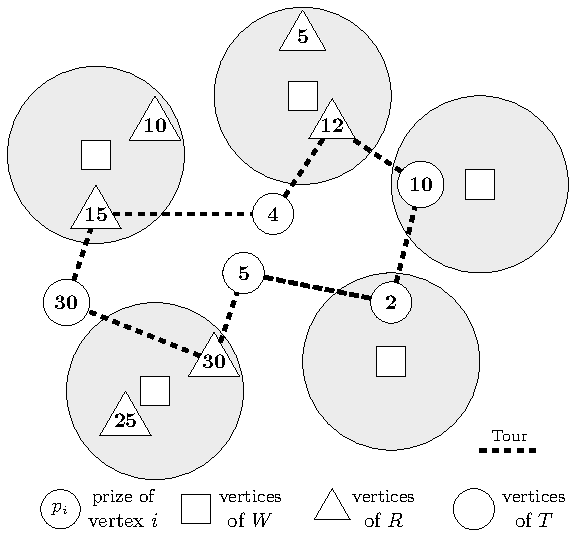
\includegraphics[width=0.45\textwidth]{pcctp-solution.pdf}
	\caption{An example of a solution for the PCCTP, adopted from \citep{daSilva}.}
	\label{fig:pcctp}
\end{figure}



A real-world application for the PCCTP can be seen in the provision of a tour for the health care project, mentioned in Section \ref{sec:intro}. The vertices from $T$ would reflect major cities in a certain region and hence be classified as required visiting points, whereas the vertices of $R$ would indicate cities where stops are optional. Moreover, there is a group of cities that should be visited, but for some reason, this is impractical. Then, their population must be served by some neighbouring cities with a distance of up to $D$ units, to avoid mass people displacement. This last set of cities would belong to $W$. In order to be worthy of releasing a vehicle, a minimum number of people must participate. As a result, the prize of each vertex represents the population of each city in $T$ and $R$, and the total \textit{PRIZE} to be collected corresponds to the minimum total number of residents to be serviced.


The new mathematical formulation proposed in this work is an undirected model that uses cut-sets, rather than flow \citep{lyra2004problema} or multi-flow \citep{silva2009problema} constraints for the sub-tour elimination. The decision variables are: $x_e =  1$, if edge  $e \in E$  is used, and 	$x_e=0$ otherwise; and  $y_i =  1,$ if vertex  $i \in R$ is visited, and $y_i=0$  otherwise.		We also define $\delta(S) = \{ (i,j) \in E \ | \ i \in S, j \in V \setminus S \}$, $\delta(i)$ as a set of all edges with an endpoint at vertex $i$, and a root vertex $u \in T$. A cover is defined as $R_w = \{ i \in V \ | \ c_{iw} \leq D \}$ for each $w \in W$, and $R_W = \bigcup_{w \in W} R_w$. The PCCTP can then be formulated as the following 0-1 integer linear program:


\begin{small}
\begin{flalign}
&\min  \displaystyle \sum_{e \in E} c_e x_e \label{eq:fo3}\\
&s.t.: \displaystyle  \sum_{e \in E} x_e= |T| + \sum_{i \in R} y_i \label{eq:r3.1}    \\
& \displaystyle \sum_{i \in R} p_i y_i \geq PRIZE  \label{eq:r3.2}\\
& \displaystyle \sum_{i \in R_w } y_i \geq 1, && \forall w \in W \label{eq:r3.3} \\
& \displaystyle \sum_{e \in \delta(i)} x_e = 2, && \forall i \in T \label{eq:r3.4} \\
& \displaystyle \sum_{e \in \delta(i)} x_e = 2 y_i, && \forall i \in R \label{eq:r3.5}\\
%		\end{flalign}
%	\columnbreak	
%		\begin{flalign}
& \displaystyle \sum_{e \in \delta(S)} x_e \geq 2, &&\forall S \subseteq V \setminus \{ u \}, S \cap T \neq  \emptyset  \label{eq:r3.6} \\
& \displaystyle \sum_{e \in \delta(S)} x_e \geq 2, &&\forall S \subseteq R, \forall w \in W, R_w \subseteq S \label{eq:r3.7} \\
& \displaystyle \sum_{e \in \delta(S)} x_e \geq 2y_t, &&\forall S \subseteq R, t \in S \label{eq:r3.8} \\
&x_e \leq y_v, &&\forall e = (i,j) \in E, v \in \{ i, j \}, v \in R \label{eq:r3.9} \\
&x_e \in \{ 0, 1 \}, &&\forall e \in E \label{eq:r3.10} \\
&y_i \in \{ 0, 1 \}, &&\forall i \in R \label{eq:r3.11}
\end{flalign}
\end{small}

The objective function (\ref{eq:fo3}) minimizes the cost of the tour.  Constraint (\ref{eq:r3.1}) ensures that the number of vertices in the tour will be equal to the number of mandatory vertices plus the number of vertices chosen from $ R $. Constraint (\ref{eq:r3.2}) imposes a minimum bound on the collected prize. Constraints (\ref{eq:r3.3}) demand that all vertices in $ W $ must be covered by at least one vertex in $V$. The degree constraints (\ref{eq:r3.4}) and (\ref{eq:r3.5}) guarantee that a feasible solution goes exactly once through each visited vertex. 

Constraints (\ref{eq:r3.6}), (\ref{eq:r3.7}), and (\ref{eq:r3.8}) are the cut-sets that hold the connectivity of the tour, and together with constraints (\ref{eq:r3.1}), (\ref{eq:r3.4}), and (\ref{eq:r3.5}) guarantee the elimination of sub-tours. Then, constraint (\ref{eq:r3.9}) associates the variables of each edge in the tour with their respective vertices, that is, if an edge is in the tour, its extreme vertices will also be. Finally, constraints (\ref{eq:r3.10}) and (\ref{eq:r3.11}) define the domain of the variables.


\section{Valid inequalities for the PCCTP}
\label{sec:valid}
We use inequalities obtained from the associated 	knapsack \citep{balas1975facets} and traveling salesman \citep{berube2009branch} polytopes and cut-set inequalities for sets of vertices that cannot contain any solution to the problem.

\subsection{Cover Inequalities}


Cover inequalities can be applied to problems whose formulations have constraints associated with the polytope of the knapsack problem \citep{balas1975facets}. If a constraint takes the form of a knapsack constraint, that is, a sum of binary variables with non-negative coefficients less than or equal to a non-negative value on the right side, then there is a minimal cover associated with this constraint \citep{wolsey2014integer}. 

From constraints (\ref{eq:r3.2}), one can define the  polytope associated with the knapsack problem as $ conv \{y \in \{0,1 \}^R \}: y \text{ satisfies (\ref{eq:r3.2})} \}$, where \textit{conv} stands for the convex hull \citep{berube2009branch}. Thus, a cover inequality for the PCCTP can be defined as follows:


\begin{flalign}
        &\displaystyle \sum_{i \in C} y_i \geq 1, & \forall C \subset R, \sum_{i \in R \setminus C} p_i < PRIZE \label{eq:dc}
\end{flalign}

For all cover found in the inequality (\ref{eq:dc}), it is guaranteed that at least one vertex of the cover is in the tour, that is, there is no way to set all variables of $ C $ to zero, and simultaneously meet the $PRIZE$. For the inequality (\ref{eq:dc}) to be strong as possible, the cover $C$ must be minimal, i.e., $ C \setminus \{j \}$ is not a cover for any $ j \in C$. Equation (\ref{eq:dc}) can be strengthened by an extension defined as:

\begin{flalign}
&\displaystyle \sum_{i \in C} y_i + \sum_{i \in \bar{C}} y_i \geq  1 + |\bar{C}|& , \forall C \subset R, \sum_{i \in R \setminus C} p_i < PRIZE  \label{eq:covercutextended} 
\end{flalign}

\noindent where $\displaystyle \bar{C} = \{ i \in R \setminus C : p_i \geq \max_{j \in C} p_j \}$ \citep{balas1975facets}.

%From the constraints (\ref{eq:r3.2}), referring to the collecting of minimum premium, it is possible to define the polytope associated with the backpack problem as $ conv \ {y \ in \ {0.1 \} ^ R \}: y $ satisfates (\ ref {eq: r3.2}) $ \} $ \ cite {berube2009branch}. Thus, a coverage cut for PRRCP can be defined as follows:


\subsection{2-Matching inequalities}
There are many valid inequalities for the TSP which can be adapted for the PCCTP \citep{junger1995traveling,naddef2007polyhedral}. Among those, we have applied the 2-matching inequalities, discovered by \citet{edmonds1965maximum} in the context of matching problems.


For any set $H \subset V$ and any edge set $\mathcal{T} \subset \delta(H)$ such that $|\mathcal{T}|=\tau$ is odd, we have:

\begin{flalign}
\displaystyle \sum_{e \in E(H)} x_e +  \sum_{e \in E(\mathcal{T})} x_e \leq | H |  + \floor*{\frac{\tau}{2}}
\end{flalign}

The set $H$ is called the \textit{handle} and the edges in $\mathcal{T}$ are called \textit{teeth} (see Figure \ref{fig:2-matching}). Since a solution for the PCCTP \textit{must} contains the vertices from set $T$, its respective variables have been considered as constants, and the 2-matching inequalities was adapted as:

\begin{small}
\begin{flalign}
&\displaystyle \sum_{e \in E(H)} x_e + \sum_{e \in E(\mathcal{T})} x_e \leq | T | + \sum_{i \in H \setminus T} y_i + \floor*{ \frac{\tau}{2} } \label{eq:2-matching}
\end{flalign}
\end{small}

\begin{figure}[h]
	\centering
	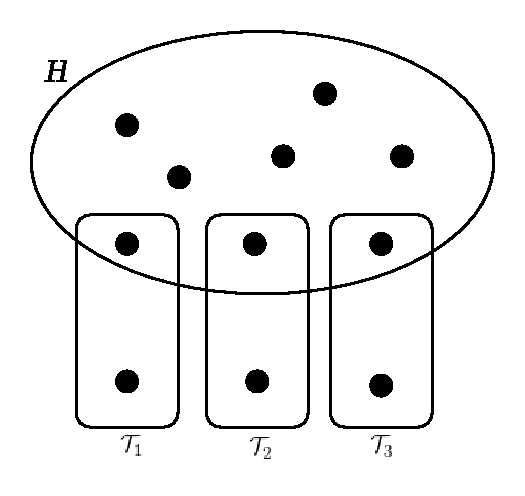
\includegraphics[width=4cm]{2-matching.pdf}
	\caption{2-matching with three teeth.}
	\label{fig:2-matching}
\end{figure}



\subsection{Cut-sets inequalities}

In this work, a new valid inequality for the PCCTP is presented,  to strengthen constraints (\ref{eq:r3.8}), in specific cases. Given a set of edges, and its respective set of vertices $S$, such that $\{u\} \notin S $, this new cut is applied when there is no possibility that the set $ V \setminus S $ contains the optimal solution. For example, if the sum of the prize associated with the vertices contained in the subset $ V \setminus S $ is less than $ PRIZE $, or if the cost of the cycle contained in the subgraph induced by $ V \setminus S $, is greater than the cost of a known solution.

In the scenario where $V \setminus S$ can not contains an optimal solution, so there must be at least two incident edges in $S$. In this way, the cut-set inequalities can be described as:

\begin{flalign}
& \displaystyle \sum_{e \in \delta(S)} x_e \geq 2 & , \forall S \subseteq R, S^* \not\subset V \setminus S, \text{ e } S^* \not\subset S   \label{eq:cutset_new}
\end{flalign}

\noindent where  $S^*$ is an optimal solution for the PCCTP.

\section{Branch-and-cut algorithm}
\label{sec:bnc}

In the model proposed in this work, (\ref{eq:r3.6}), (\ref{eq:r3.7}), and (\ref{eq:r3.8}) represent  an exponential number of
cut-set constraints. Hopefully, such constraints can be verified in polynomial time, allowing us to use a branch-and-cut approach. In this section, we introduce an exact B\&C for the PCCTP considering the formulation (\ref{eq:fo3})-(\ref{eq:r3.11}).

As is usually done in the literature, the set of exponential size constraints (\ref{eq:r3.6}), (\ref{eq:r3.7}), and (\ref{eq:r3.8}), are initially relaxed, that is, its integrality constraints are dropped \citep{doi:10.1504/IJISE.2018.094841}. Next, after the iteration of each LP, one checks if the current LP's solution violates any of them. If this is the case, the discovered violated constraints are included into the current relaxation, and a stronger relaxation is solved.

For solving the LP relaxations and handling the search tree, we have used the Mixed Integer Programming (MIP) solver Gurobi \citep{gurobi}. Therefore, the aforementioned approach has been included into an enumeration scheme that applies it not just to the enumeration tree's root node, but also to all generated nodes.


In the following, we describe the separation procedures used in our B\&C algorithm to identify violated inequalities from Sections \ref{sec:models} and \ref{sec:valid}. To this end, consider $G^*=(V^*,E^*)$ 
as a graph induced by an optimal solution $S=(x^*,y^*)$  to the current relaxation, in which  $V^* = \{i \in V : y_i^* > 0\}$ and $E^* = \{e \in E : x_e^* >0 \}$.

\subsection{Cut-sets}
For constraints  (\ref{eq:r3.6}), let $x^*_e$ be a capacity value associated with every edge $e \in E$.
Regardless of whether $S$ is integer or fractional, the cut-set constraints are separated, and for both cases, we have proceeded as follows. A minimum ($u, i$)-cut is found in $G^*$ by means of a maximum-flow/min-cut algorithm for  any $i \in T\setminus\{u\}$; if it yields a value less than $2$, a violated constraint is found. Thus, one incorporates  this constraint to the model and solve it again. For the min-cut algorithm, one used the pre-flow push algorithm presented in \citet{ciupala2008preflow} which performs in $O(|V|^2 \sqrt{|E|})$ for each vertex, and therefore, with an overall worst-case complexity of $O(|V|^3 \sqrt{|E|})$ to find a violated cut-set.



The separation of constraints (\ref{eq:r3.7}) and (\ref{eq:r3.8}) was carried out in a similar way to the aforementioned separation, but with different subsets of vertices that participate in the maximum-flow algorithm. In the constraints (\ref{eq:r3.7}), for every $w \in W$ a special vertex $\bar{v}$ was created, and for every $i \in R_w$ an edge $(i,\bar{v})$ with capacity $c_{i,\bar{v}}=2$ was generated. The idea of inserting $\bar{v}$ is to find a minimum capacity cut in $G^*$, between every  $(u,\bar{v})$ pair. Thus,  this separation algorithm has a complexity of  $O(|W||V|^2\sqrt{|E|})$.

Lastly, for constraints (\ref{eq:r3.8}), for every $i \in R^* \subset V^*: y_i > 0$, one finds a minimum capacity cut $(u,i)$ in $G^*$, if the output is less than $2y_i$, there is a violated constraint. Therefore, this separation algorithm is  $O(|R||V|^2\sqrt{|E|)})$.

\subsection{Cover inequalities}
%\citet{crowder1983solving} noted that cover inequalities can be rewritten as ${\textstyle \sum_{j \in C} (1-y_j) \geq 1}$, so its separation is equivalent to the following knapsack-type problem:

%\begin{flalign}
%&\displaystyle min \sum_{j \in N} (1-y_j^*)z_j& \\
%&\displaystyle s.a: \sum_{j \in N} p_j z_j \geq b + 1& \\
%&\displaystyle z_j \in \{0,1\}, &\forall j \in N
%\end{flalign}

For separating the cover inequalities, we have adopted the idea of \citet{crowder1983solving}, by inserting items (vertices) into $C$ in non-decreasing order of $-y_j/p_j$ until a cover is obtained. This heuristic takes $O(n log_n)$ time. As soon as a minimal cover is obtained, the extension process will be carried out. This process consists of creating an extension $\bar{C}$, containing all vertices of $R\setminus C$ with prizes equal to or greater than $max \{p_j: j \in C\}$.


\subsection{2-Matching inequalities}

These inequalities, when applied to the PCCTP, can be separated in polynomial time, by simply modifying the exact separation algorithm proposed by \citet{padberg1982odd}. However, in order to reduce the computational effort demanded by this exact algorithm, in this work, the heuristic proposed by \citet{fischetti1998solving} was used.

Consider $ x_e^*$ as weights associated with the edges. The method of \citet {fischetti1998solving} consists of applying a Kruskal's greedy algorithm \cite {gower1969minimum} to find a minimum cost spanning tree in $ G^*$. At each iteration in which this algorithm selects a new edge $e$, is defined (in the sub-graph of $G^*$ induced by all selected edges so far), a connected component containing $e$, called handle ($ H $). The node set $H$ is then considered as the handle of a hopefully violated 2-matching constraint. For any $ H $, the tooth edges are optimally determined by the following procedure. Let $\delta (H) = \{e_1, ..., e_ \tau \}$ such that $x_ {e1}^* \geq x_ {e2}^* \geq ... \geq x_ {e \tau}^*$. Initially, the constraint that the teeth must be disjointed at vertices is relaxed, and for any $ | \mathcal{T} | \geq 3$ and odd, the best choice for $ \mathcal{T} $ consists of the edges $ e_1, ... e_\tau$. Therefore, a most-violated 2-matching inequality lies in choosing an odd number of teeth, $ |\mathcal{T}| \geq 3 $, in which maximize:

{\footnotesize
\begin{flalign}
x_{e1}^* + (x_{e2}^* + x_{e3}^* - 1) + ... + (x_{e\tau-1}^* + x_{e\tau}^* - 1) 
\end{flalign}
}
	
If no violated cut can be produced in this fashion, then  no violated 2-matching constraint exists for the given $ H $. Otherwise, there is a violated 2-matching constraint and, if two tooth edges, $e$ and $ f $, overlap on a $ v $ node, then one simplifies the inequality by defining a new pair handle-tooth ($ H ', \mathcal {T}' $) with $ \mathcal{T}'\gets \mathcal{T} \setminus \{e, f\}$ and, $ H'\gets H \setminus \{v \} $ (if $ v \in H $) or $ H' \gets H \cup \{v \} $ (if $ v \notin H $). According to \citet{fischetti1998solving}, the iteration of this simplification step always results in a violated 2-matching constraint with non-overlapping teeth.
				
In some cases, this procedure can even lead to a 2-matching constraint with $ | \mathcal{T} | = 1 $; if this occurs, we reject the inequality in favor of a cut-set associated with the handle.


\section{Reduction rules}

\label{sec:rules}

\citet{lyra2004problema} and \citet{silva2009problema} have proposed six reduction rules for the PCCTP. Such rules are preprocessing procedures that aim to reduce the search space by removing edges or vertices, and not affecting the finding of optimal solutions. 


Some reduction rules of the literature and proposed in this work, assumed that  the costs $c_{ij}$ satisfy the triangle inequality, therefore, for every rule presented from this assumption, we have placed the symbol $\triangle$ at the beginning. Moreover,  consider the vertices in $W$ covered by a vertex  $i \in V$ as $R_i = \{ w \in W \ | \ c_{iw} \leq D \}$. The reduction rules presented in the literature are: 

%\begin{footnotesize}
 \begin{itemize}
	\item \textbf{R1}: If $\exists w \in W$, where $|R_w| = 1$, then $T = T \cup R_w$;
	
	\item \textbf{R2}: If $\exists j \in R$, where $p_j > 0$ and $\sum_{i \in V \setminus \{ j \}} p_i < PRIZE$, then $T = T \cup \{ j \}$;
	
	\item \textbf{R3}: If $\triangle$ and $\sum_{i \in T}p_i \geq PRIZE$, then all the vertices from $R \setminus R_W$ can be removed from $G$, if the resulting graph of this removal is complete in relation to $T \cup R_W$;
	
	\item \textbf{R4}: If $\triangle$, $ \sum_{i \in T}p_i \geq PRIZE$ and $\exists i \in R$ where $R_i \subseteq \bigcup_{t \in T} R_t$, then one can  remove the vertex $i$ from $G$, if the resulting graph of this removal is complete;
	
	
	\item \textbf{R5}: If $\triangle$, $\exists$ $i,j \in R$, $i \neq j$, $ \sum_{k \in V \setminus \{i \}} p_k \geq PRIZE$, $R_i \subseteq R_j$, $c_{ik} > c_{jk}$ $\forall k$ adjacent to $i$, and $\exists$ $(v_1,v_2) \in E$ $\forall$ $(i,v_1)$ e $(i,v_2) \in E$, then one can remove the vertex $i$ from $G$;
	
	
	\item \textbf{R6}: If $\exists t \in T$, such that $R_t \neq \emptyset$, then $W = W \setminus R_t$;
	
	\item \textbf{R7}: If $\exists w \in W$ such that $R_w = R$ then $W = W \setminus \{ w \}$, and at least one vertex from $R$ must be in the tour.
	
\end{itemize}	
%\end{footnotesize}








 In this work, we propose the following six new reduction rules:


%\begin{footnotesize}

\begin{itemize}
% 	\item \textbf{R8}: If $\triangle$, $r \in R\setminus R_W$ and ($PRIZE  \leq 0$ or $p_r=0$), then $R = R \setminus \{ r \}$ and $\forall (i,r), (j,r) \in \delta(r)$ $c_{ij} = \min (c_{ij}, (c_{ir} + c_{rj}))$. In case $(i,j) \notin E$,  we add $(i,j)$ in $E$ with cost $c_{ir} + c_{rj}$;

%	\textcolor{red}{troquei $\sum_{i \in T} p_i \geq PRIZE$ por ($PRIZE  \leq 0$ ou $p_r=0$), já que escrevemos que apenas os vértices opcionais tem prêmio associado.}

\item  \textbf{R8}: (A generalisation of rules \textbf{R3} and \textbf{R4} from \citet{lyra2004problema}). If $\triangle$, and $\exists$ $r \in R$ such that $p_r = 0$ or $PRIZE \leq 0$, $\exists$ $v \in R$ where $R_r \subseteq R_v$ and $\forall (r,i), (r,j) \in \delta(r)$,  $i,j \in V \setminus \{ v \}$ and $i \neq j$ $c_{ir} + c_{rj} \geq c_{iv} + c_{vj}$ and $c_{ij} \leq c_{ir} + c_{rj}$, then $R = R \setminus \{ r \}$, as long as  the graph resulting from this removal is complete in relation to $T$;


%	Caso $(i,j) \notin E$ então usamos $c_{ij} = \infty$;

\item  \textbf{R9}: If $\exists r \in R$ such that in $G' = (V', E')$, where $V' = V \setminus \{ r \}$ and $E' = E \setminus \delta(r)$, there are no two disjoint paths at vertices between two terminal vertices, a terminal and no vertex of $ R_w $, $ w \in W $, or between any pair of vertices $ i, j $ where $ i \in R_w $ and $ j \in R _ {\bar{w}} $, $ w \neq \bar{w} $ and $ w, \bar{w} \in W $, then $ T = T \cup \{r \} $;

\item \textbf{R10}: If $ \exists r_1, r_2 \in R $ such that $ G'= (V', E ')$, in which $ V' = V \setminus \{r_1, r_2 \} $ and $ E'= E \setminus (\delta(r_1) \cup \delta (r_2))$, is disconnected; Each connected component of $ G'$ is defined by $ G'_i = (V'_i, E'_i) $, $ i \in \{1, \ldots nc \} $. If $ \nexists i \in \{1, \ldots nc \} $ such that $ T \subseteq V'_i $, $ V'_i \cap R_w \neq \emptyset $ $ \forall w \in W $, and $ \sum_ {i \in V'_i} p_i \geq PRIZE $, then $ T = T \cup \{r_1, r_2 \} $;


\item \textbf{R11}: If $\exists i \in T$, where $p_i > 0$ then $PRIZE = PRIZE - p_i$ e $p_i = 0$.


\item \textbf{R12}: If $\exists i \in V$ such that $|\delta(i)| \leq 1$, then $V = V \setminus \{ i \}$. Note that if $i \in T$, then the problem is unfeasible;

\item \textbf{R13}: If $\exists w, w' \in W$, $w \neq w'$, such that $R_{w'} \subseteq R_w$, then $W = W \setminus \{ w \}$.
\end{itemize}
%\end{footnotesize}


%As regras apresentadas por  \citet{lyra2004problema} e  \citet{silva2009problema} foram propostas considerando a hipótese  que os custos $c_{ij}$ satisfazem a desigualdade triangular, ou seja, $\forall (i,j) \in E$ e $k \in V \setminus \{i,j\}$, $c_{ij} \leq c_{ik} + c_{kj}$. Portanto, neste trabalho, toda regra aplicada a partir dessa hipótese possuirá o símbolo $\triangle$ no início. 


\section{The hybrid heuristic }
\label{sec:heristics}

Since the PCCTP is NP-Hard \citep{lyra2004problema}, we also propose a  new hybrid heuristic (MPO\_S), that combines ILP  with the state-of-the-art heuristic GRASP-GENIUS-RVND \citep{daSilva}.


\subsection{GRASP-GENIUS-RVND}
The GRASP-GENIUS-RVND \citep{daSilva} is based on the GRASP (Greedy Randomised Adaptive Search Procedure) metaheuristic \citep{grasp03}. GRASP is based on a multi-start strategy, in which many initial solutions are generated through repeated applications of a semi-greedy process. At each multi-start iteration, given a constructed solution $S$, its neighbourhood $N(S)$ is explored by a local search, in order to find a better solution. The iterative process of performing the two phases, initial solution generation, and local search, is interrupted according to a stopping criterion, which can be a maximum number of interactions, a target solution value, or timeout.



% The GRASP metaheuristic is executed iteratively, and each iteration is composed of two phases: construction and local search. A feasible solution $S$ is generated in the construction phase, and then its neighbourhood $N(S)$ is explored by a local search, in order to find a better solution. This iterative process is repeated until a stop criterion is reached, which can be a limited number of iterations, a number of iterations without solution improvement, among others. The best solution found in all iterations $S^*$ is returned.

\citet{daSilva} developed the solution generation phase based on the GENIUS heuristic \citep{genius} adapted for the PCCTP, while in the other phase, some moves were devised and combined in an RVND (Random Variable neighbourhood Descent) framework \citep{mladenovic97}.


\subsubsection{GENIUS}

The GENIUS heuristic \citep{genius} is implemented with  two steps: a construction approach, the GENI step (Generalized Insertion), and an improvement procedure, the Unstringing and Stringing (US) step. 

GENI is method with a generalized insertion. Its main feature is that the evaluation of possible insertion of vertices is basically not limited to the positions between consecutive vertices.
The US step involves removing a vertex from the tour and reinserting it in another position, in each iteration, to improve the current solution. When there are no more possibilities for improvement, this process stops.

% The GENI is a generalized insertion-based method whose main characteristic is that the evaluation of the possible insertions of a vertex is not essentially limited to a position between consecutive vertices. 
% The US step consists, at each iteration, of removing
% one vertex from the tour and re-inserting it in another position with a view
% of improving the current solution. This procedure stops when there is no more
% possibility of improvements.

In the construction phase, we start by randomly selecting three vertices from $T$ to generate a partial tour. Then, as long as there are vertices of $T$ outside the tour, the $PRIZE$ has not been reached, and there are any uncovered vertices $w \in W $, we  perform the following steps: i) create a candidate list (CL), which contains all vertices outside the tour; ii) obtain a restricted candidate list (RCL) which is composed of the best quality vertices from CL; iii) a vertex is randomly selected from RCL and inserted in the tour by a GENIUS procedure; iv) try to improve the tour by applying the US method. The pseudo-code of the GENIUS process is given in the algorithm \ref{alg:genius_PCCTP}.

According to \citet{daSilva}, if the incremental cost of a vertex is lower than the threshold $c^{min} + (\alpha \times (c^{max}-c^{min}))$, the vertex is inserted into in the RCL, in which $c^{min}$ and $c^{max}$ are the smallest and largest incremental costs in CL, respectively. The greedy parameter $\alpha \in [0,1]$ represents the greedy degree of the heuristic, the lower the value of $\alpha$ is, the lower the greedy.

% For calculating the incremental cost, we used the following greedy function, which considers the insertion of a vertex $k$ between vertices $i$ and $j$.

We have used the greedy function below to calculate the incremental cost, which takes into account the insertion of a vertex $k$ between vertices $i$ and $j$.

\begin{flalign}
g(k) = \displaystyle \min_{i,j \in V : i \neq j} \left(c_{ik} + c_{kj}  - c_{ij}\right) \label{custo_inc}
\end{flalign}

\noindent where $c_{ij}$, $c_{ik}$ and $c_{kj}$ are the costs of the edges $(i,j)$, $(i,k)$ and $(k,j)$, respectively.

\begin{algorithm}[ht]
	%	\algsetup{linenosize=\scriptsize}
	\caption{\hspace{-1mm}: GENIUS($seed$,$\alpha$)}
	\label{alg:genius_PCCTP}
	%	{\footnotesize
		{\footnotesize
	\begin{algorithmic}[1]
		%			\REQUIRE $seed$, $\alpha$
		\STATE $i, j, k \gets \texttt{SelectRandom}(T,seed)$;
		\STATE $S \gets \cup$ $\{i, j, k\}$;
% 		\STATE $CL \gets V$;
		\STATE $CL \gets V \setminus \{i,j,k\}$
		\WHILE{$(\exists$ $t \in T$ : $t \notin S )$ \textbf{or} $(\exists$ not covered $w \in W\space)$ \textbf{or} (\textit{PRIZE} not collected) }
		\STATE $RCL \gets \texttt{setRCL}(CL, \alpha)$;
		\STATE $v \gets \texttt{SelectRandom}(RCL,seed)$;
		\STATE $GENI(S,v)$;
		\STATE $CL \gets CL \backslash {v} $;
		\ENDWHILE
		\STATE $US(S)$; \textit{//tour improvement}\\
		\RETURN $S$;
	\end{algorithmic}
		}
\end{algorithm}

\subsubsection{RVND}
Following the GRASP construction phase, the generated solution is subjected to a local search using the Random VND technique \citep{SUBRAMANIAN20101899}. The VND is a local search metaheuristic proposed by \citet{mladenovic97} that employs several neighbourhood structures. Given an ordered list of neighbourhoods, initially, the VND explores the first neighbourhood of $S$, $N^k(S)$, and if a better solution cannot be discovered, the next $N^{(k + 1)}(S) $  neighbourhood is investigated. Otherwise, it will go back to the first neighbourhood on the list. When all neighbourhood structures have been explored, the algorithm comes to a halt and returns the best solution found. For their heuristic, \citet{daSilva} used the RVND instead of the traditional VND in which there is no neighbourhood order.


% After the construction phase of GRASP, the built solution goes through a local search performed by the Random VND method \citep{SUBRAMANIAN20101899}. Proposed by \citet{mladenovic97}, the VND is a local search metaheuristic that uses different neighbourhood structures. Given an ordered list of neighbourhoods, the VND starts by exploring the first neighbourhood of $S$, $N^k(S)$, and if a better solution is not found, the next neighbourhood $N^{(k + 1)}(S) $ is explored. Otherwise, it returns to the first neighbourhood on the list. The algorithm stops when all neighbourhood structures are explored, returning the best solution found. In this work, we have used the RVND instead of the conventional VND, where there is no ordering of neighbourhoods. 


The RVND is detailed in the pseudo-code of Algorithm \ref{alg:vnd}, and it starts by shuffling the list of neighbourhood structures. Then, we can see that the counter $k$ is incremented by one to try the next neighbourhood if the current solution is not improved.
Otherwise, the current neighbourhood's local optimal solution is achieved, and $k$ is set back to 1 for restarting the loop for the newly accepted solution.
When there is no chance of improving $S$, that is, $k > k_{max}$, one returns the best current solution.

RVND is described in detail in the pseudo-code of Algorithm \ref{alg:vnd}. It first scrambles the list of neighbourhood structures. Then, we can see that if the current solution is not improved, the counter $k$ will increase by 1 to try the next neighbourhood. Otherwise, we obtain the local optimal solution of the current neighbourhood and we set $k$ to 1 to restart the loop for the newly accepted solution. When there are no neighbors to improve $S$, that is, $k> k_{max}$, the algorithm returns the current best solution.



% For the RVND, we used  the 15 neighbourhood structures presented in \citet{daSilva}, which are based on classical movements for the TSP as \textit{swap} and \textit{shift}, and heuristics as GENIUS and Cheapest Insertion.

For RVND, we have used the 15 neighbourhood structures introduced in \citet{daSilva}, which are based on TSP's classic movements \textit{swap} and \textit{shift}, as well as heuristics as GENIUS and the cheapest insert.


\begin{algorithm}
	\caption{\hspace{-1mm}: RVND($S, N$)}
	\label{alg:vnd}
		{\footnotesize
	\begin{algorithmic}[1]		
		\STATE  Set a random order for the neighbourhood structures in $N$	
		\STATE $k \gets 1$
		\WHILE {$k \leq k\_max$}
		\STATE $S' \gets firstImprovingSolution(N^{(k)}(S))$;
		\IF{\textit{S' is better than S}}
		\STATE $S \gets S'$;
		\STATE $k \gets 1$;
		\ELSE
		\STATE $k \gets k + 1$;
		\ENDIF
		\ENDWHILE
		\RETURN $S$
	\end{algorithmic}	
}
\end{algorithm}

\subsection{MPO\_S}
%grammar check here

%In the last decades, there have been several reports of positive experiences with the combination of classical metaheuristic components and other techniques such as integer linear programming (ILP) and data mining to provide robust hybrid heuristics \citep{blum2008hybrid}.

% In \citet{climaco2018}, the authors proposed a hybrid method created from the combination of an approach based on the GRASP metaheuristic with ILP, called MPO. Its main idea is to identify some promising/unpromising edges during the base heuristic process, fix/remove their respective variable from the ILP model, and then solve it. This process intends to accelerate the resolution of the modified problem without loss of solution quality, regarding the best solution reached by the original heuristic.

In \citet{climaco2018}, the authors presented a hybrid approach, which was created by combining GRASP meta-heuristics and ILP-based methods, called MPO. Its main idea is to identify some promising/unpromising edges in the basic heuristic process, repair/remove their respective variables from the ILP model, and then solve it. This process aims to speed up the resolution of the modified problem without losing the quality of the solution, concerning the best solution achieved by the original heuristic method.


From an analysis of the exe\-cu\-tions of its heuristic, \citet{climaco2018} realized that several edges had never been chosen for a local optimal solution along with the iterations. For all test instances, at least 70\% of $E$ had never been present in any solutions reached. Thus, these unpromising edges (denoted as $E^0$) were removed in order to reduce the search space induced by $G$. In this work, we have done this same analysis with the GRASP-GENIUS-RVND heuristic proposed by \citet{daSilva}. We have found that, on average, the size of $E^0$ is about 88\%. The result of this last analysis motivated us to build our hybrid approach based on the strategy of \citet{climaco2018}.

In preliminary experiments, we also realized that from certain iterations, the set $E^0$ was not undergoing modifications. Thus, we determined that the heuristic process may be interrupted as soon as the $E^0$ set becomes stable - which means no change in the $E^0$ set occurred throughout a given number of iterations. This interruption may save us some processing time, and we would create an $E^0$ set of practically the same quality as if all the iterations had been performed.
                                          
\citet{climaco2018} fixed in their model part of the solution obtained by the base heuristic, in order to further reduce the search space, under the hypothesis that the heuristic and exact model were making similar decisions since their solutions shared several edges in common. We hypothesized that only with the removal of $E^0$ set, we would already have a satisfactory acceleration of our ILP model, therefore, this last strategy was not adopted in our approach.
                                          
The pseudo-code of our hybrid approach, denoted as MPO\-\_S, is presented in Algorithm \ref{alg:mpo}. In line 1, we initialize some variables and constants, including the $E^0$ as the set $E$ itself. In line 2 the constant $stable$ represents the number of iterations without change that the $E^0$ must have, to be considered as stable; this constant is initialized as $\gamma$ times the maximum iterations of the heuristic process ($maxIt$), in which $\gamma \in \mathbb{R}$ such that $0 \leq \gamma \leq 1$. From lines 3 to 19, the GRASP-GENIUS-RVND heuristic is described with some extra instructions, for the construction of the set $E^0$ and its interruption if $E^0$ set becomes stable. If the set $E^0$ is not stable at any time, the heuristic will be executed for $maxIt$ iterations.
                                          
 In line 4, the procedure GENIUS generates a feasible solution, and then, in line 5, the neighbourhood of this solution is explored by the RVND. From lines 6 to 8, if $S'$ is better than the best current solution $S^*$, then the best solution is updated. In line 9 the function \texttt{update()} removes all edges $e \in S'$ from $E^0$. As output, the variable \textit{flag} receives \textit{false} if no edge was removed from $E^0$, and $true$ otherwise. From lines 10 to 13, a counter is incremented if in the current iteration the set $E^0$ was not changed. Lines 15 to 17 interrupt the heuristic process if the set $E^0$ has not been modified for the number of needed iterations.
                                          
 Once the heuristic is interrupted or performed the maximum number of iterations, the model is modified in line 19. The respective variable $x_e$ of each $e \in E^0$ is removed from the model. Finally, in line 20 the modified model is solved and the final solution is returned in line 21.
                                          
\begin{algorithm}[!h]
	\caption{\hspace{-1mm}: \textbf{MPO\_S}($maxIt,\alpha, seed, \gamma, model$)}
	\label{alg:mpo}
		{\footnotesize
	\begin{algorithmic}[1]		
		\STATE $S^*\gets \emptyset$; $f(S^*) \gets \infty$; $E^0 \gets E$; $count \gets 0$; $flag \gets false$; 
		\STATE $stable \gets \gamma \times maxIt$; 
		\FOR{$k=1$ \TO $k \leq maxIt$}
		\STATE $S \gets \texttt{GENIUS} (\alpha, seed)$;  \COMMENT{Construction phase}
		\STATE $S' \gets \texttt{RVND} (S,\alpha, seed)$; \COMMENT{Local search phase}
		\IF{$f(S') \leq f(S^*)$}
		\STATE $S^* \gets S'$;
		\ENDIF
		%	\STATE $k \gets k +1$;
		\STATE $flag \gets \texttt{update}(S',E^0)$;
		\IF{$flag \neq true$}
		\STATE $count \gets count + 1$;
		\ELSE
		\STATE $count \gets 0$;
		\ENDIF
		\IF{$count = stable$}
		\STATE break; \COMMENT{here the heuristic process is interrupted}
		\ENDIF
		\ENDFOR
		
		\STATE $model \gets $ \texttt{remove}($E^0$, $model$);
		\STATE $S^* \gets $ \texttt{solve}($model$);
		\RETURN $S^*$;
	\end{algorithmic}
}
\end{algorithm}


\section{Computational results}
\label{sec:results}

% In this section, the computational results obtained for the proposed strategies are reported and compared to the state-of-the-art heuristic GRASP-GENIUS-RVND for the PCCTP \citep{daSilva}.

All formulations and heuristics presented were implemented in \textit{C++} language and compiled with \textit{g++ 5.4.0}. The experiments were carried out on an Intel(R) Core i7-6700 CPU\@ 3.40GHz machine with 16GB of RAM. For the implementation and execution of the formulations, the mathematical solver Gurobi (version 6.5.2) was used with its cuts, pre-processing and heuristics disable. Besides, a one-hour processing time limit was determined, and the parallelization capability of the processor has been disabled. 

This section starts with a description of the PCCTP
instances used for the experiments. Next, we present the results for the mathematical formulations along with the impact of the applied valid inequalities on these formulations. Results for the reduction rules and their impact on the mathematical formulations follow. Finally, results of the hybrid approach are reported.

%We remark that the source-code of the GRASP-GENIUS-RVND was kindly provided by its author \citep{daSilva}, and we have kept all parameters of the heuristic, excepting for the $maxIt$, which we will explain later.

 
\subsection{Instances}

The benchmark instances utilised in this study were introduced in \citet{silva2009problema}, and contains  144 test problems adapted from the travelling salesman problem (TSP),  which can be found in the TSPLIB repository \citep{reinelt1991tsplib}. Note that the \textit{PRIZE} is never satisfied by collecting prizes just from $T$ in order to prevent any instance of the PCCTP from becoming an instance of the covering tour problem (CTP).

These instances given new names according to their original name in the TSPLIB, together with information about the subsets $R$, $T$, $W$ and the percentage of prize to be collected, in respect to the total available prize. The instance \textit{brazil58\_R18\_T20\_W20\_25}, for example, contains the following properties: a total of 58 vertices; 18 of them are optional($R$); 20 are mandatory ($T$); 20 of them must be covered ($W$); and 25\% of the total instance prize must be collected. The whole instance set are publicly available at \url{http://www.deinf.ufma.br/~glaubos/papers/instances/pcctp.zip}.


\subsection{Results for the mathematical formulations}
This section presents comparisons between the results obtained by the two formulations of the literature, flow \citep{lyra2004problema} and multi-flow \citep{silva2009problema}, and the proposed branch-and-cut (B\&C) algorithm. 

Table \ref{tab:models} shows the results obtained by executing these exact approaches. The first column refers to the name of the instances, and the second column presents the best-known solution reported in the literature (either optimal or heuristic). From the third column, the solution value and the time spent (in seconds) by each approach are presented. Moreover, the fields with ``-'' indicate that, due to the time exceeded by one hour of processing, or problems related to lack of memory, it was not possible to solve the respective instance. The values in bold indicate the best results in running time and the best solution found.


Only the 50 cases that provide the greatest variations in performance between the formulations, either in solution quality or CPU time, were chosen for clarity and readability. The complete results of this experiment are available at \url{www.deinf.ufma.br/~glaubos/PCCTP_complete_results.pdf}.



\begin{table*}
	\centering
	\caption{Results obtained by the Flow and Multi-flow formulations, and the B\&C}
	\label{tab:models}
	{\footnotesize
	\begin{tabular}{lcrrrrrr}
		\hline
		& \multicolumn{1}{l}{} & \multicolumn{2}{c}{Flow \citep{lyra2004problema}} & \multicolumn{2}{c}{Multi-flow \citep{silva2009problema}}          & \multicolumn{2}{c}{B\&C}         \\
		\cline{2-8}
		\multicolumn{1}{c}{Instance} & BKS & Sol. & T. (s) & \multicolumn{1}{c}{Sol.} & \multicolumn{1}{c}{T. (s)} & Sol. & \multicolumn{1}{c}{T. (s)} \\
		\hline
		rat99\_R19\_T60\_W20\_75    & 1017                 & -               & 3600.0 & \multicolumn{1}{l}{-} & 3600.0          & \textbf{1017}  & \textbf{1.0}    \\
		eil101\_R19\_T61\_W21\_50   & 506                  & 1547            & 3600.0 & \multicolumn{1}{l}{-} & 3600.0          & \textbf{506}   & \textbf{4.4}    \\
		gr120\_R24\_T72\_W24\_50    & 5159                 & -               & 3600.0 & \multicolumn{1}{l}{-} & 3600.0          & \textbf{5159}  & \textbf{6.6}    \\
		lin105\_R21\_T63\_W21\_50   & 11583                & 58498           & 3600.0 & \multicolumn{1}{l}{-} & 3600.0          & \textbf{11583} & \textbf{15.0}   \\
		si175\_R59\_T58\_W58\_75    & 8402                 & -               & 3600.0 & \multicolumn{1}{l}{-} & 3600.0          & \textbf{8402}  & \textbf{96.2}   \\
		kroA100\_R20\_T60\_W20\_50  & 16544                & -               & 3600.0 & \multicolumn{1}{l}{-} & 3600.0          & \textbf{16544} & \textbf{96.5}   \\
		bier127\_R24\_T77\_W26\_25  & 98453                & -               & 3600.0 & \multicolumn{1}{l}{-} & 3600.0          & \textbf{98453} & \textbf{140.2}  \\
		kroB100\_R34\_T33\_W33\_75  & 14768                & 25197           & 3600.0 & \multicolumn{1}{l}{-} & 3600.0          & \textbf{14768} & \textbf{150.7}  \\
		pr107\_R35\_T36\_W36\_75    & 37292                & 57482           & 3600.0 & \multicolumn{1}{l}{-} & 3600.0          & \textbf{37292} & \textbf{291.7}  \\
		kroE100\_R34\_T33\_W33\_75  & 14622                & 27385           & 3600.0 & \multicolumn{1}{l}{-} & 3600.0          & \textbf{14622} & \textbf{690.3}  \\
		kroA200\_R40\_T40\_W120\_75 & 15197                & -               & 3600.0 & \multicolumn{1}{l}{-} & 3600.0          & \textbf{15197} & \textbf{2188.9} \\
		gr137\_R26\_T28\_W83\_25    & 39305                & 59114           & 3600.0 & 60630                 & 3600.0          & \textbf{39305} & \textbf{270.6}  \\
		pr144\_R28\_T29\_W87\_50    & 30294                & 82642           & 3600.0 & \textbf{30294}        & \textbf{408.0}  & 33433          & 3600.0          \\
		st70\_R22\_T24\_W24\_75     & 505                  & 826             & 3600.0 & 540                   & 3600.0          & \textbf{505}   & \textbf{1.6}    \\
		pr124\_R24\_T25\_W75\_75    & 34359                & 62995           & 3600.0 & 36719                 & 3600.0          & \textbf{34359} & \textbf{11.1}   \\
		kroC100\_R34\_T33\_W33\_50  & 13235                & 40281           & 3600.0 & \textbf{13235}        & \textbf{1796.3} & 13563          & 3600.0          \\
		rat99\_R33\_T33\_W33\_50    & 847                  & 1196            & 3600.0 & 863                   & 3600.0          & \textbf{847}   & \textbf{3.6}    \\
		pr76\_R24\_T26\_W26\_50     & 74539                & 116859          & 3600.0 & \textbf{74539}        & \textbf{1012.3} & 75594          & 3600.0          \\
		pr152\_R29\_T31\_W92\_75    & 49110                & 70971           & 3600.0 & 49167                 & 3600.0          & \textbf{49110} & \textbf{39.0}   \\
		si175\_R35\_T35\_W105\_25   & 4845                 & 9941            & 3600.0 & \textbf{4845}         & 1960.3          & \textbf{4845}  & \textbf{0.3}    \\
		eil51\_R9\_T31\_W11\_75     & 348                  & 484             & 3600.0 & \textbf{348}          & 909.6           & \textbf{348}   & \textbf{0.4}    \\
		eil76\_R14\_T46\_W16\_25    & 387                  & 612             & 3600.0 & \textbf{387}          & 1135.7          & \textbf{387}   & \textbf{0.6}    \\
		gr120\_R40\_T40\_W40\_25    & 4301                 & 17438           & 3600.0 & \textbf{4301}         & 1929.8          & \textbf{4301}  & \textbf{2.8}    \\
		u159\_R31\_T32\_W96\_50     & 28613                & 47566           & 3600.0 & \textbf{28613}        & 606.4           & \textbf{28613} & \textbf{1.3}    \\
		eil101\_R33\_T34\_W34\_75   & 462                  & 1367            & 3600.0 & \textbf{462}          & 3600.0          & \textbf{462}   & \textbf{8.6}    \\
		eil101\_R19\_T21\_W61\_25   & 356                  & 433             & 3600.0 & \textbf{356}          & 285.6           & \textbf{356}   & \textbf{0.8}    \\
		brazil58\_R11\_T12\_W35\_75 & 20466                & \textbf{20466}  & 3600.0 & \textbf{20466}        & 53.7            & \textbf{20466} & \textbf{0.2}    \\
		berlin52\_R9\_T32\_W11\_75  & 6916                 & 6994            & 3600.0 & \textbf{6916}         & 92.7            & \textbf{6916}  & \textbf{0.3}    \\
		eil76\_R24\_T26\_W26\_50    & 338                  & 775             & 3600.0 & \textbf{338}          & 252.3           & \textbf{338}   & \textbf{1.0}    \\
		ch150\_R30\_T30\_W90\_75    & 4292                 & 10981           & 3600.0 & \textbf{4292}         & 513.7           & \textbf{4292}  & \textbf{2.5}    \\
		kroE100\_R20\_T20\_W60\_50  & 10586                & 12260           & 3600.0 & \textbf{10586}        & 551.7           & \textbf{10586} & \textbf{2.8}    \\
		berlin52\_R16\_T18\_W18\_50 & 5186                 & 5484            & 3600.0 & \textbf{5186}         & 463.4           & \textbf{5186}  & \textbf{3.0}    \\
		att48\_R9\_T29\_W10\_50     & 2824                 & 3040            & 3600.0 & \textbf{2824}         & 52.9            & \textbf{2824}  & \textbf{0.3}    \\
		pr107\_R20\_T22\_W65\_50    & 35869                & 47333           & 3600.0 & \textbf{35869}        & 65.7            & \textbf{35869} & \textbf{0.5}    \\
		ch130\_R26\_T26\_W78\_50    & 4139                 & -               & 3600.0 & \textbf{4139}         & 296.0           & \textbf{4139}  & \textbf{2.3}    \\
		rd100\_R20\_T20\_W60\_75    & 5421                 & 6705            & 3600.0 & \textbf{5421}         & 143.4           & \textbf{5421}  & \textbf{1.1}    \\
		st70\_R14\_T14\_W42\_25     & 419                  & 474             & 3600.0 & \textbf{419}          & 42.6            & \textbf{419}   & \textbf{0.3}    \\
		hk48\_R9\_T29\_W10\_25      & 9708                 & 10557           & 3600.0 & \textbf{9708}         & 50.5            & \textbf{9708}  & \textbf{0.4}    \\
		rat99\_R19\_T20\_W60\_25    & 792                  & 1362            & 3600.0 & \textbf{792}          & 12.8            & \textbf{792}   & \textbf{0.1}    \\
		gr96\_R18\_T20\_W58\_75     & 30015                & 34379           & 3600.0 & \textbf{30015}        & 467.1           & \textbf{30015} & \textbf{5.1}    \\
		eil51\_R17\_T17\_W17\_25    & 273                  & \textbf{273}    & 2666.8 & \textbf{273}          & 94.6            & \textbf{273}   & \textbf{1.3}    \\
		brazil58\_R11\_T35\_W12\_50 & 23312                & 32029           & 3600.0 & \textbf{23312}        & 109.6           & \textbf{23312} & \textbf{1.8}    \\
		gr120\_R24\_T24\_W72\_75    & 4275                 & 9702            & 3600.0 & \textbf{4275}         & 139.7           & \textbf{4275}  & \textbf{2.3}    \\
		bier127\_R24\_T26\_W77\_50  & 74745                & 125855          & 3600.0 & \textbf{74745}        & 495.2           & \textbf{74745} & \textbf{8.9}    \\
		eil76\_R14\_T16\_W46\_75    & 332                  & \textbf{332}    & 1525.2 & \textbf{332}          & 24.5            & \textbf{332}   & \textbf{0.4}    \\
		att48\_R16\_T16\_W16\_75    & 2650                 & 3012            & 3600.0 & \textbf{2650}         & 30.6            & \textbf{2650}  & \textbf{0.6}    \\
		pr76\_R14\_T46\_W16\_75     & 90862                & 219818          & 3600.0 & \textbf{90862}        & 523.3           & \textbf{90862} & \textbf{12.6}   \\
		hk48\_R16\_T16\_W16\_50     & 7593                 & \textbf{7593}   & 3381.7 & \textbf{7593}         & 17.1            & \textbf{7593}  & \textbf{0.5}    \\
		gr48\_R16\_T16\_W16\_25     & 3571                 & \textbf{3571}   & 1608.0 & \textbf{3571}         & 10.9            & \textbf{3571}  & \textbf{0.5}    \\
		kroC100\_R20\_T20\_W60\_75  & 12582                & 15900           & 3600.0 & \textbf{12582}        & 78.4            & \textbf{12582} & \textbf{3.6}   \\
		\hline
	\end{tabular}
}
\end{table*}

In the literature, results of the formulations of \citet{lyra2004problema} and \citet{silva2009problema} are presented, but with different instances. Therefore, in Table \ref{tab:models}, unpublished results of the flow formulation \citep{lyra2004problema} are presented for the instances proposed in the work of \citet{silva2009problema}. 

Considering the whole set of instances, the flow formulation \citep{lyra2004problema} was able to achieve optimal solutions in only 6.94\% of the instances, while the formulation of \citet{silva2009problema}, based on multi-flow constraints, finds optimal solutions in 34.72\% of the cases. From Table \ref{tab:models}, it is clear that the B\&C solves several instances not solved by formulations of the literature, within the time-limit of one hour; and, even when another formulation solves the instance, the B\&C does it much faster. 

Considering all the 144 instances, we can see that, regarding the number of optimal solutions found, the B\&C approach outperformed the others, reaching an optimal solution in 56\% of cases and proving unprecedented optimality for 12 instances, solved only by heuristics so far. We remark that the optimal values obtained for these new instances, are the same values already obtained by the heuristics from the literature. Regarding the processing time spent, the superiority of B\&C remained. On average, the new exact approach reduced the CPU time of the multi-flow formulation by 43\%, demanding more time in just four cases.

\subsubsection{Impact of the valid inequalities}

After the experiment with the formulations, an experiment was carried out to verify the impact of applying the new proposed inequalities  (\ref{eq:covercutextended}, \ref{eq:2-matching} and \ref{eq:cutset_new}) together with the B\&C.

Table \ref{tab:cuts} presents the results in which the application of inequalities reduced the time to solve the problem, and complete results are available at \url{www.deinf.ufma.br/~glaubos/PCCTP_complete_results.pdf}. The first column indicates the instances used. The second column shows the CPU-time spent by the B\&C with the valid inequalities. The third column presents the CPU-time spent by the B\&C without the valid inequalities. The fourth column shows the CPU-time percentage difference between the B\&C with and without the application of the inequalities. To calculate this difference, we used Equation (\ref{eq:time}). Finally, the last column ``New?'' indicates whether new optimal solutions have been found or not.

We would like to remark that since the Gurobi is a ``black-box'' type of framework, many implementation details are hidden from the users and one of them is how the user cuts are managed or even if all of them are used.

{\footnotesize
\begin{flalign}
Dif_T = 100 \times \frac{(B\&C - B\&C \text{ }ineq)}{B\&C} \label{eq:time}
\end{flalign}
}
\begin{table}[h]
	\centering
	\caption{Results of applying the valid inequalities along with the proposed  branch-and-cut}
	\label{tab:cuts}
	
	{\footnotesize
		
	\begin{tabular}{l@{\hspace{0.4\tabcolsep}}r@{\hspace{0.4\tabcolsep}}r@{\hspace{0.4\tabcolsep}}r@{\hspace{0.4\tabcolsep}}c}
		\hline
		Instance & \multicolumn{1}{l}{\begin{tabular}[c]{@{}l@{}}B\&C\\ ineq\end{tabular}} & \multicolumn{1}{c}{B\&C} & \multicolumn{1}{c}{$Dif_T$} & New? \\
		\hline
		brazil58\_R18\_T20\_W20\_25 & 8.3    & 801.4  & 99.0 & No           \\
		d198\_R39\_T40\_W119\_25    & 47.2   & 3600.0 & 98.7 & \textbf{Yes} \\
		kroA100\_R34\_T33\_W33\_75  & 51.8   & 3600.0 & 98.6 & \textbf{Yes} \\
		kroC100\_R34\_T33\_W33\_50  & 64.9   & 3600.0 & 98.2 & \textbf{Yes} \\
		gr96\_R32\_T32\_W32\_50     & 17.4   & 945.2  & 98.2 & No           \\
		gil262\_R51\_T53\_W158\_25  & 68.3   & 3600.0 & 98.1 & \textbf{Yes} \\
		kroB150\_R30\_T30\_W90\_25  & 74.3   & 3600.0 & 97.9 & \textbf{Yes} \\
		kroB100\_R20\_T60\_W20\_25  & 81.2   & 3600.0 & 97.7 & \textbf{Yes} \\
		rd100\_R34\_T33\_W33\_25    & 89.6   & 3600.0 & 97.5 & \textbf{Yes} \\
		gr96\_R18\_T58\_W20\_25     & 12.9   & 418.0  & 96.9 & No           \\
		pr76\_R24\_T26\_W26\_50     & 134.4  & 3600.0 & 96.3 & \textbf{Yes} \\
		gr137\_R26\_T28\_W83\_25    & 13.6   & 270.6  & 95.0 & No           \\
		gr137\_R26\_T83\_W28\_75    & 185.9  & 3600.0 & 94.8 & \textbf{Yes} \\
		pr107\_R35\_T36\_W36\_75    & 18.4   & 291.7  & 93.7 & No           \\
		kroE100\_R20\_T60\_W20\_25  & 36.4   & 370.3  & 90.2 & No           \\
		tsp225\_R45\_T45\_W135\_75  & 75.1   & 658.3  & 88.6 & No           \\
		kroC100\_R20\_T60\_W20\_25  & 33.2   & 278.7  & 88.1 & No           \\
		kroE100\_R34\_T33\_W33\_75  & 93.8   & 690.3  & 86.4 & No           \\
		kroA200\_R40\_T40\_W120\_75 & 300.3  & 2188.9 & 86.3 & No           \\
		lin105\_R21\_T21\_W63\_25   & 3.1    & 22.0   & 85.8 & No           \\
		pr136\_R26\_T82\_W28\_75    & 742.8  & 3600.0 & 79.4 & \textbf{Yes} \\
		berlin52\_R16\_T18\_W18\_50 & 1.0    & 3.0    & 66.1 & No           \\
		ch150\_R50\_T50\_W50\_25    & 211.0  & 511.8  & 58.8 & No           \\
		kroA150\_R30\_T90\_W30\_75  & 1502.4 & 3600.0 & 58.3 & \textbf{Yes} \\
		si175\_R59\_T58\_W58\_75    & 40.3   & 96.2   & 58.1 & No           \\
		eil76\_R14\_T16\_W46\_75    & 0.2    & 0.4    & 56.8 & No           \\
		pr152\_R29\_T31\_W92\_75    & 18.7   & 39.0   & 52.2 & No           \\
		berlin52\_R9\_T11\_W32\_25  & 0.1    & 0.1    & 41.7 & No           \\
		kroA100\_R20\_T20\_W60\_25  & 7.5    & 12.5   & 39.8 & No           \\
		u159\_R31\_T96\_W32\_25     & 2275.4 & 3600.0 & 36.8 & \textbf{Yes} \\
		kroA100\_R20\_T60\_W20\_50  & 62.3   & 96.5   & 35.5 & No           \\
		u159\_R53\_T53\_W53\_75     & 187.8  & 290.2  & 35.3 & No           \\
		brg180\_R36\_T108\_W36\_75  & 81.7   & 123.4  & 33.8 & No           \\
		pr136\_R46\_T45\_W45\_50    & 2396.7 & 3600.0 & 33.4 & \textbf{Yes} \\
		pr136\_R26\_T28\_W82\_25    & 17.6   & 24.3   & 27.5 & No           \\
		hk48\_R9\_T10\_W29\_75      & 0.0    & 0.0    & 25.0 & No           \\
		kroB100\_R34\_T33\_W33\_75  & 114.9  & 150.7  & 23.8 & No           \\
		gr96\_R18\_T20\_W58\_75     & 4.0    & 5.1    & 21.6 & No           \\
		gr120\_R24\_T24\_W72\_75    & 1.8    & 2.3    & 18.9 & No           \\
		kroB100\_R34\_T33\_W33\_50  & 3062.1 & 3600.0 & 14.9 & \textbf{Yes} \\
		brazil58\_R11\_T35\_W12\_50 & 1.6    & 1.8    & 10.7 & No      \\
		\hline    
	\end{tabular}
}
\end{table}


From Table \ref{tab:cuts}, one can see that we manage to solve 14 more instances, in relation to the application of the branch-and-cut without the inequalities. The new solution values obtained in these instances are the same as in the experiment without applying the inequalities. However, we can now state that they correspond to optimal solution values, as the time limit has not been reached. Without these inequalities, the solver times out at 3600 seconds, not being able to prove optimality.

Considering all 144 instances, it is observed that the application of valid cuts enhances the B\&C, especially for larger instances such as d198\_\-R39\_\-T40\_\-W119\_25, kroA150\_\-R30\_\-T90\_\-W30\_75, and gil262\_\-R51\_\-T53\_\-W158\_\-25. In terms of CPU time spent, the solver had a modest speedup of 0.3\% and  was impaired or benefited depending on the instance, but when benefited, the time gain was quite significant. In some cases, the time reduction was about 90\%.

\subsection{Results for the reduction rules}
\label{sec:regras}

\citet{silva2009problema} and \citet{lyra2004problema} applied their reduction rules in the sequence that they are presented in Section \ref{sec:rules}. However, before verifying its impact on reducing the input problem, an investigation was carried out on what would be the best order to apply them.

The impact of applying the rules depends on the graph that represents the problem. By removing the set $E^0 $, there is a sparse version of the graph that was originally complete. Therefore, with this investigation, we also sought to find the application sequences that best fit each graph version.

For the design of the sequences, the following scenario was considered: i) some rules will have a random order of application because, by the definition of the instances, it is hard to establish the ideal position for its call; ii) some rules will have ``fixed predecessors'', as it has been observed that these rules are likely to have a greater impact if executed after certain other rules; and, half of the sequences will be designed to favour a greater reduction in the original graph of the instances, and the other half in more sparse graphs (after removing $ E^0$). The proposed sequences were as follows:

{\footnotesize
	\begin{enumerate}[A:]
		
		\item  R6, R2, R13, R5, R8, R7, R3, R10, R9, R4, R1, R13, R11;  
		
		\item  R6, R5, R2, R13, R7, R8, R4, R13, R1, R9, R10, R3, R11; 
		
		\item  R9, R10,  R11, R1, R3, R8, R2, R4, R6,R7,R12, R5, R13, R8;
		
		\item  R10, R3, R9, R11, R1, R4, R8, R6,R2, R7, R5, R13, R12;
		
		\item R2, R10, R3, R11, R1, R4, R9, R8, R6,   R7, R5, R13, R12;
		
		\item R6, R9, R2, R10, R12, R11, R1, R5, R3, R8, R4, R7, R13.
		
	\end{enumerate}
}


\subsubsection{Reduction on complete graphs}
After defining the application sequences, experiments were carried out with the 37 test-instances. The first experiment with the rules was performed over a complete graph, that is, $G=(V,E)$ without removing the set $E^0$.

Table \ref{tab:sum-rr-complete}  summarises the complete results for the aforementioned experiment, which are available at \url{http://www.deinf.ufma.br/~glaubos/PCCTP_complete_results.pdf}. For each set of vertices $ R, T $ and $ W $, the columns show the average difference ($ \Delta $) between the number of vertices before, and after  applying the rules, and the average time spent by each sequence.
The ``+'' symbol indicates an increase in the number of vertices, while the ``-'' represents a reduction.

The application of rules R10 and R11 is more expensive than the others, and they are not able to make any reduction in complete graphs. Thus, at the beginning of each rule R10 and R11, it is verified if the input graph is complete. If so, then the rule is not applied. 


\begin{table}[!h]
	\centering
	\caption{Summary for reduction rules results on complete graphs}
	\label{tab:sum-rr-complete}
	{\footnotesize
	\begin{tabular}{lrrrr}
		\hline
		 & Avg. $\Delta$ |R|     & Avg. $\Delta$ |T|     & Avg. $\Delta$ |W|      & Avg. T (s)     \\
		\hline
		A        & -4.46          & \textbf{+3.00} & -44.65          & 36.541         \\
		B        & -3.00          & \textbf{+3.00} & -44.65          & 36.924         \\
		C        & \textbf{-4.97} & \textbf{+3.00} & \textbf{-49.35} & \textbf{0.001} \\
		D        & \textbf{-4.97} & \textbf{+3.00} & \textbf{-49.35} & \textbf{0.001} \\
		E        & \textbf{-4.97} & \textbf{+3.00} & \textbf{-49.35} & 33.440         \\
		F        & -4.49          & \textbf{+3.00} & -44.65          & 35.445       \\
		\hline 
	\end{tabular}
}
\end{table}

From Table \ref{tab:sum-rr-complete}, one can observe that 'C', 'D', and 'E' are the rules that most impact the reduction of the graph, employing an average reduction of 57.32 vertices per instance. Among these rules, 'C' and 'D' are the fastest, requiring on average less than 0.01 seconds per instance.

In terms of processing time, the sequences with the best performance were those in which R10 and R11 were one of the first three rules applied. In the other sequences, the rules that precede R10 and R11 reduce some vertices, making the graph incomplete and allowing the application of R10 and R11. However, the reductions in the rules that precede R10 and R11, do not leave the graph sparse enough to compensate for the time spent by these last two rules.

The set $ W $ is by far the more affected among the vertex sets, so the sequences that reduced the vertices the most (`C', `D' and `E') were the ones that reduced the most vertices $ w \in W $. The rule that, on average, reduced vertices the most was R6 (removes $ w \in W $ covered by $ t \in T $) which, in all three sequences with the most reductions, was preceded by rule R1 (moves $ r \in R $ to $ T $).

 Rule R1 is the only one that precedes R6 and makes some kind of reduction. So, it was hypothesized that this precedence is the reason why sequences `C', `D', and `E' outperform the others. Considering the aforementioned observations, it was defined that the sequences `C' and `D' are the best when it comes to applying the rules in complete graphs.
% The results of this experiment are shown in Tables \ ref {tab: rr-a-b}, \ ref {tab: rr-c-d} and \ ref {tab: rr-e-f}, located in the appendix of this thesis.

\subsubsection{Reduction on sparse graphs}

Experiments were performed using the same sequences A, B, C, D and E, but now for more sparse graphs. For such an experiment, the GRASP-GENIUS-RVND was executed only once for each test instance, with $\gamma = 0.10$. After calling the heuristic and constructing the set $ E^0 $, all edges of $ E^0 $ were removed from the graph that represents the instance, originally complete.

With this edge removal, there is a more sparse graph than the original and therefore more susceptible to reductions. Thus, as in the case of complete graphs, the results with sparse graphs have been summarized (see Table \ref{tab:sum-rr-sparse}), and the complete results are available at \url{http://www.deinf.ufma.br/~glaubos/PCCTP_complete_results.pdf}.

\begin{table}[!h]
	\centering
	\caption{Summary for reduction rules results on sparse graphs}
	\label{tab:sum-rr-sparse}
	{\footnotesize
	\begin{tabular}{lrrrr}
		\hline
		& Avg. $\Delta$ |R| & Avg. $\Delta$ |T| & Avg. $\Delta$ |W| & Avg. T (s) \\
		\hline
	A & \textbf{-7.08} & \textbf{+4.78} & -44.73          & 5.28          \\
	B & -7.05          & +4.70          & -44.73          & 5.26          \\
	C & -6.20          & +2.08          & -45.87          & 2.38          \\
	D & -7.04          & +2.77          & \textbf{-49.40} & \textbf{2.06} \\
	E & -7.04          & +2.77          & \textbf{-49.40} & 3.68          \\
	F & -5.70          & +3.05          & -44.73          & 4.13         \\
		\hline    
	\end{tabular}
}
\end{table}

For sparse graphs, the average number of reduced vertices increased in most sequences: 'A' went from 52.11 to 56.65; 'B' went from 50.65 to 56.49; 'C' went from 57.32 to 54.15; 'D' went from 57.32 to 59.21; 'E' went from 57.32 to 59.21; and 'F' went from 52.14 to 53.49. In this last experiment, the performance of the sequences was more balanced than the experiment with complete graphs and, again, the sequences that made the most reductions in the set $W$ had better performance. The sequences that most reduced vertices were 'D' and 'E', on average 59.21 vertices. Between these two sequences, sequence 'D' was the faster, with an average time of 2.60 seconds.  

\subsubsection{Impact of reduction rules on the mathematical formulations}
In this section, we report the impact of applying the reduction rules R1 to R14 on the three mathematical formulations presented in this work. To this end, experiments were carried out applying the sequence 'D' on the input graph of each formulation. Table \ref{tab:rr-exact},  summarises all the solution improvements that occurred with the application of the rules. The first column identifies the instance in which the improvement occurred, and in the second column, for each formulation, the cost of the solution without applying the rules is presented, followed by the new cost obtained with the application. The symbol ``*'' indicates that the obtained value is optimal and ``- '' indicates that no solution was obtained within the time limit of one hour. The complete results of this experiments are available at \url{www.deinf.ufma.br/~glaubos}.

\begin{table}[!h]
	\centering
	\caption{Impact of reduction rules on exact approaches (solution quality)}
	\label{tab:rr-exact}
	{\footnotesize
	\begin{tabular}{lr}
		\hline
		Instance                   & Flow \citep{lyra2004problema}                            \\
		\hline
		rat99\_R19\_T20\_W60\_25   & 1362 / 792$^*$   \\
		st70\_R14\_T14\_W42\_25    & 474 / 419$^*$     \\
		&                                  \\
		\hline
		Instance                   & Multi-flow \citep{silva2009problema}                       \\
		\hline
		gr137\_R26\_T28\_W83\_25   & 60630/ 39305$^*$  \\
		lin105\_R21\_T63\_W21\_50  & - / 11583$^*$                       \\
		lin105\_R35\_T35\_W35\_75  & 11090 / 10566$^*$ \\
		pr107\_R20\_T65\_W22\_25   & - / 40994$^*$                       \\
		pr107\_R35\_T36\_W36\_75   & - / 37292$^*$                       \\
		pr152\_R29\_T31\_W92\_75   & 49167/ 49110$^*$                    \\
		rat99\_R19\_T60\_W20\_75   & - / 1017$^*$      \\
		st70\_R22\_T24\_W24\_75    & 540/505$^*$       \\
		kroA100\_R20\_T60\_W20\_50 & - / 16544$^*$     \\
		eil101\_R33\_T34\_W34\_75  & 462 / 462$^*$     \\
		&                                  \\
		\hline
		Instance                   & B\&C                             \\
		\hline
		kroA150\_R30\_T90\_W30\_75 & 21976/ 21974* 
	\end{tabular}
}
\end{table}

From Table \ref{tab:rr-exact}, it is noted that the reduction rules performed before calling the solver, improve the solution quality for some instances. In the flow formulation \citep{lyra2004problema}, the number of solved instances was increased by two and, on average, its CPU-time was reduced by 3.20\%. The Multi-Flow formulation \citep{silva2009problema}, which was unable to solve several cases due to problems related to lack of memory, was the formulation most benefited by the application of the rules. The formulation of \citet{silva2009problema} obtained an increase of ten solved instances, while its CPU-time was reduced on average, 19.10\%. Finally, in the proposed B\&C approach, there was a new solved instance and an average reduction of 15.75\% in its processing time.

\subsection{Results for the MPO\_S}
\label{sec:mpo}

%Originally, the GRASP-GENIUS-RVND \citep{daSilva} heuristic was developed to be finished as soon as a certain target solution value was reached, or within a predefined maximum running time. Since the MPO\_S heuristic process requires a maximum number of iterations, in this work, experiments were carried out with 37 test-instances, which represented as much as possible the characteristics of the entire set.
%For each TSPLIB \citep{reinelt1991tsplib} instance size, \citet{silva2009problema} generated three instances for the PCCTP; then, for the tuning experiments, one instance of each size was selected, and instances with similar sizes (difference less than five vertices) were rejected.

Since we aim to demonstrate the efficiency of our approach compared to the state-of-the-art heuristic, in our experiments with the MPO\_S, we have maintained the parameters of the GRASP-GENIUS-RVND ($\alpha = 0.6$ and $maxIt = 70 $) and used the model proposed in this work. Therefore, the only parameter we have tuned is the $\gamma$. Also, the time-limit established for the solver was reduced to 1800 seconds, since it has never been reached inside of the MPO\_S with the 37 test-instances.

%Considering the original stop criteria, it was found that on average, the GRASP-GENIUS-RVND performs 70 iterations. Therefore, for the heuristic process contained within the MPO\_S, the parameter $ maxIt $ was defined as 70. Also, the parameter $ \alpha = 0.6 $ has been maintained since it has already been tuned in \citet{daSilva}.

\subsubsection{The $\gamma$ parameter}

For tuning the $\gamma$ parameter, experiments were carried out with 37 test-instances, which represent as much as possible the characteristics of the entire set. For each TSPLIB \citep{reinelt1991tsplib} instance size, \citet{silva2009problema} generated three instances for the PCCTP; then, for the tuning experiment, one instance of each size was selected, and instances with similar sizes (difference less than five vertices) were rejected.

First, we have randomly tried different values of $\gamma$ in the range $[0,1]$, and we  observed that, as the value of $ \gamma $ decreased, the $E^0 $ was considered stable faster and the heuristic phase was interrupted in a smaller number of iterations. Then, for a better estimation of the value of $ \gamma $, an empirical analysis of the MPO\_S executions was conducted on the 37 test-instances. Such analysis tested $\gamma \in \{0.05, 0.10, 0.15, 0.20\}$ and the results are shown in Tables \ref{gamma-5-10-15} and \ref{gamma-20}.

% Please add the following required packages to your document preamble:
% \usepackage{graphicx}
\begin{table*}[h]
\caption{Results for MPO\_S with $\gamma= 0.05, 0.10$ and $0.15$}
\label{gamma-5-10-15}
\footnotesize{%
\begin{tabular}{lrrrrrrrrr}
\hline
                            & \multicolumn{3}{c}{$\gamma=0.05$} & \multicolumn{3}{c}{$\gamma=0.10$} & \multicolumn{3}{c}{$\gamma=0.15$} \\
                            \cline{2-10}
Instance &
  \multicolumn{1}{c}{\begin{tabular}[c]{@{}c@{}}Best \\ Sol.\end{tabular}} &
  \multicolumn{1}{c}{\begin{tabular}[c]{@{}c@{}}Avg.\\ Sol.\end{tabular}} &
  \multicolumn{1}{c}{\begin{tabular}[c]{@{}c@{}}Avg.\\ T.(s)\end{tabular}} &
  \multicolumn{1}{c}{\begin{tabular}[c]{@{}c@{}}Best \\ Sol.\end{tabular}} &
  \multicolumn{1}{c}{\begin{tabular}[c]{@{}c@{}}Avg.\\ Sol.\end{tabular}} &
  \multicolumn{1}{c}{\begin{tabular}[c]{@{}c@{}}Avg.\\ T.(s)\end{tabular}} &
  \multicolumn{1}{c}{\begin{tabular}[c]{@{}c@{}}Best \\ Sol.\end{tabular}} &
  \multicolumn{1}{c}{\begin{tabular}[c]{@{}c@{}}Avg.\\ Sol.\end{tabular}} &
  \multicolumn{1}{c}{\begin{tabular}[c]{@{}c@{}}Avg.\\ T.(s)\end{tabular}} \\
  \hline
att48\_R9\_T10\_W29\_25     & 2291    & 2291.2    & 0.2     & 2291    & 2291.0    & 0.3      & 2291    & 2291.0    & 0.0      \\
berlin52\_R9\_T11\_W32\_25  & 4861    & 4862.4    & 0.2     & 4861    & 4861.0    & 0.3      & 4861    & 4861.0    & 0.0      \\
bier127\_R24\_T77\_W26\_25  & 98597   & 98597.0   & 96.0    & 98453   & 98453.0   & 94.2     & 98453   & 98453.0   & 19.8     \\
brazil58\_R18\_T20\_W20\_25 & 19417   & 19417.0   & 3.3     & 19417   & 19417.0   & 6.4      & 19417   & 19417.0   & 1.9      \\
brg180\_R36\_T36\_W108\_25  & 550     & 550.0     & 24.3    & 550     & 550.0     & 23.9     & 550     & 550.0     & 2.0      \\
ch130\_R44\_T43\_W43\_25    & 4383    & 4383.9    & 5.7     & 4383    & 4383.0    & 15.4     & 4383    & 4383.0    & 0.1      \\
ch150\_R50\_T50\_W50\_25    & 4778    & 4799.0    & 23.4    & 4778    & 4790.0    & 50.2     & 4778    & 4785.0    & 0.4      \\
d198\_R39\_T40\_W119\_25    & 10916   & 10916.0   & 1829.2  & 10916   & 10916.0   & 1830.0   & 10916   & 10916.0   & 1800.1   \\
eil51\_R17\_T17\_W17\_25    & 273     & 273.3     & 0.6     & 273     & 273.0     & 1.2      & 273     & 273.0     & 0.1      \\
eil76\_R14\_T46\_W16\_25    & 387     & 387.0     & 3.6     & 387     & 387.0     & 5.9      & 387     & 387.0     & 0.0      \\
eil101\_R19\_T21\_W61\_25   & 356     & 356.0     & 1.7     & 356     & 356.0     & 3.6      & 356     & 356.0     & 0.1      \\
gr48\_R16\_T16\_W16\_25     & 3571    & 3571.0    & 0.2     & 3571    & 3571.0    & 0.5      & 3571    & 3571.0    & 0.0      \\
gr96\_R18\_T58\_W20\_25     & 42746   & 42746.0   & 33.2    & 42746   & 42746.0   & 38.5     & 42746   & 42746.0   & 6.4      \\
gr120\_R40\_T40\_W40\_25    & 4301    & 4301.0    & 9.3     & 4301    & 4301.0    & 16.9     & 4301    & 4301.0    & 0.0      \\
gr137\_R26\_T28\_W83\_25    & 39305   & 39305.0   & 1815.6  & 39305   & 39305.0   & 1815.9   & 39305   & 39305.0   & 1800.0   \\
hk48\_R9\_T29\_W10\_25      & 9708    & 9710.4    & 1.2     & 9708    & 9708.6    & 2.3      & 9708    & 9708.0    & 0.0      \\
kroA100\_R20\_T20\_W60\_25  & 10848   & 10848.0   & 3.6     & 10848   & 10848.0   & 5.4      & 10848   & 10848.0   & 0.1      \\
kroA150\_R50\_T50\_W50\_25  & 14382   & 14453.2   & 209.4   & 10535   & 10546.2   & 204.7    & 10535   & 10549.4   & 148.2    \\
kroB100\_R20\_T60\_W20\_25  & 18406   & 18406.0   & 1813.7  & 18406   & 18406.0   & 1824.6   & 18406   & 18406.0   & 1800.0   \\
kroB150\_R30\_T30\_W90\_25  & 11467   & 11477.8   & 299.3   & 11467   & 11477.8   & 268.8    & 11467   & 11476.7   & 233.4    \\
kroC100\_R20\_T60\_W20\_25  & 16785   & 16785.0   & 28.8    & 16785   & 16785.0   & 290.1    & 16785   & 16785.0   & 218.3    \\
kroE100\_R20\_T60\_W20\_25  & 17199   & 17201.5   & 14.6    & 17199   & 17199.0   & 33.6     & 17199   & 17199.0   & 27.7     \\
lin105\_R21\_T21\_W63\_25   & 8893    & 8893.0    & 6.0     & 8893    & 8893.0    & 7.9      & 8893    & 8893.0    & 0.2      \\
pr76\_R14\_T16\_W46\_25     & 66007   & 66007.0   & 0.7     & 66007   & 66007.0   & 1.3      & 66007   & 66007.0   & 0.0      \\
pr107\_R20\_T65\_W22\_25    & 40994   & 40994.0   & 386.0   & 40994   & 40994.0   & 394.8    & 40994   & 40994.0   & 0.5      \\
pr124\_R42\_T41\_W41\_25    & 35465   & 35465.0   & 1860.7  & 35465   & 35465.0   & 1861.8   & 35465   & 35465.0   & 1800.1   \\
pr136\_R26\_T28\_W82\_25    & 47620   & 47620.0   & 4.9     & 47620   & 47620.0   & 8.6      & 47620   & 47620.0   & 0.0      \\
pr144\_R28\_T87\_W29\_25    & 46940   & 46940.2   & 1634.0  & 46940   & 46940.0   & 1634.8   & 46940   & 46940.0   & 1800.1   \\
pr152\_R50\_T51\_W51\_25    & 50667   & 50667.2   & 1872.8  & 50667   & 50667.0   & 1876.3   & 50667   & 50667.3   & 1800.1   \\
rat99\_R19\_T20\_W60\_25    & 792     & 792.0     & 1.1     & 792     & 792.0     & 6.3      & 792     & 792.0     & 0.0      \\
rd100\_R34\_T33\_W33\_25    & 5552    & 5552.0    & 9.6     & 5484    & 5486.4    & 17.4     & 5484    & 5486.4    & 1.2      \\
si175\_R35\_T35\_W105\_25   & 4845    & 4845.0    & 70.0    & 4845    & 4845.0    & 70.6     & 4845    & 4845.0    & 0.0      \\
st70\_R14\_T14\_W42\_25     & 419     & 419.0     & 0.8     & 419     & 419.0     & 2.4      & 419     & 419.0     & 0.1      \\
u159\_R31\_T96\_W32\_25     & 35442   & 35442.0   & 67.8    & 35442   & 35442.0   & 86.0     & 35442   & 35442.0   & 0.0      \\
gr229\_R45\_T46\_W138\_25   & 61278   & 61307.3   & 1881.4  & 61278   & 61304.3   & 1878.2   & 61278   & 61304.3   & 1800.1   \\
pr264\_R52\_T53\_W159\_25   & 27693   & 27693.0   & 1929.9  & 27693   & 27693.1   & 1935.5   & 27693   & 27693.0   & 1799.2   \\
ts225\_R45\_T45\_W135\_25   & 87889   & 87889.0   & 48.1    & 87889   & 87889.0   & 46.5     & 87889   & 87889.0   & 0.3     \\
\hline
\end{tabular}%
}
\end{table*}

\begin{table}[h]
\caption{Results for MPO\_S with $\gamma=0.20$}
\label{gamma-20}
\begin{tabular}{lrrr}
\hline
                            & \multicolumn{3}{c}{$\gamma=0.20$} \\
                            \cline{2-4}
Instance &
  \begin{tabular}[c]{@{}l@{}}Best \\ Sol.\end{tabular} &
  \begin{tabular}[c]{@{}l@{}}Avg.\\ Sol.\end{tabular} &
  \begin{tabular}[c]{@{}l@{}}Avg.\\ T.(s)\end{tabular} \\
  \hline
att48\_R9\_T10\_W29\_25     & 2291    & 2291.0    & 0.8      \\
berlin52\_R9\_T11\_W32\_25  & 4861    & 4861.0    & 0.9      \\
bier127\_R24\_T77\_W26\_25  & 98453   & 98453.0   & 98.7     \\
brazil58\_R18\_T20\_W20\_25 & 19417   & 19417.0   & 5.9      \\
brg180\_R36\_T36\_W108\_25  & 550     & 550.0     & 23.7     \\
ch130\_R44\_T43\_W43\_25    & 4383    & 4383.0    & 21.5     \\
ch150\_R50\_T50\_W50\_25    & 4778    & 4785.0    & 58.4     \\
d198\_R39\_T40\_W119\_25    & 10916   & 10916.0   & 1852.4   \\
eil51\_R17\_T17\_W17\_25    & 273     & 273.0     & 2.6      \\
eil76\_R14\_T46\_W16\_25    & 387     & 387.0     & 12.1     \\
eil101\_R19\_T21\_W61\_25   & 356     & 356.0     & 7.7      \\
gr48\_R16\_T16\_W16\_25     & 3571    & 3571.0    & 1.8      \\
gr96\_R18\_T58\_W20\_25     & 42746   & 42746.0   & 36.4     \\
gr120\_R40\_T40\_W40\_25    & 4301    & 4301.0    & 27.4     \\
gr137\_R26\_T28\_W83\_25    & 39305   & 39305.0   & 1815.6   \\
hk48\_R9\_T29\_W10\_25      & 9708    & 9708.0    & 3.8      \\
kroA100\_R20\_T20\_W60\_25  & 10848   & 10848.0   & 5.5      \\
kroA150\_R50\_T50\_W50\_25  & 10535   & 10549.4   & 259.6    \\
kroB100\_R20\_T60\_W20\_25  & 18406   & 18406.0   & 1829.7   \\
kroB150\_R30\_T30\_W90\_25  & 11467   & 11476.7   & 233.8    \\
kroC100\_R20\_T60\_W20\_25  & 16785   & 16785.0   & 236.7    \\
kroE100\_R20\_T60\_W20\_25  & 17199   & 17199.0   & 56.9     \\
lin105\_R21\_T21\_W63\_25   & 8893    & 8893.0    & 7.9      \\
pr76\_R14\_T16\_W46\_25     & 66007   & 66007.0   & 2.6      \\
pr107\_R20\_T65\_W22\_25    & 40994   & 40994.0   & 33.6     \\
pr124\_R42\_T41\_W41\_25    & 35465   & 35465.0   & 1860.9   \\
pr136\_R26\_T28\_W82\_25    & 47620   & 47620.0   & 11.0     \\
pr144\_R28\_T87\_W29\_25    & 46940   & 46940.0   & 1888.5   \\
pr152\_R50\_T51\_W51\_25    & 50667   & 50667.3   & 1880.5   \\
rat99\_R19\_T20\_W60\_25    & 792     & 792.0     & 6.3      \\
rd100\_R34\_T33\_W33\_25    & 5484    & 5486.4    & 17.5     \\
si175\_R35\_T35\_W105\_25   & 4845    & 4845.0    & 70.9     \\
st70\_R14\_T14\_W42\_25     & 419     & 419.0     & 2.4      \\
u159\_R31\_T96\_W32\_25     & 35442   & 35442.0   & 86.5     \\
gr229\_R45\_T46\_W138\_25   & 61278   & 61304.3   & 1878.8   \\
pr264\_R52\_T53\_W159\_25   & 27693   & 27693.0   & 1937.7   \\
ts225\_R45\_T45\_W135\_25   & 87889   & 87889.0   & 46.8    \\
\hline
\end{tabular}
\end{table}

For each instance, ten executions were executed with different seeds. The results showed that with $ \gamma = 0.15 $ and $ \gamma = 0.20 $, the heuristic part of MPO\_S has always performed the maximum number of iterations, so $ \gamma$ values greater than 0.20 have not been tested since the set $ E^0$ would never stabilize. For both $\gamma$ values, 0.15 and 0.20, the MPO\_S was able to improve the best solutions found by the GRASP-GENIUS-RVND in three instances, and its average solution in 11 of them. However, the extra processing time spent by the solver did not compensate for the gain in solution quality.

The MPO\_S with $ \gamma = 0.05 $ was executed in a lower CPU-time than GRASP-GENIUS-RVND for 22 instances. However, this configuration did not allow a good construction of the set $E^0$, and as a consequence, some promising edges were erroneously removed from the model, and the solver was not able to achieve good quality solutions. None of the best solutions found by the GRASP-GENIUS-RVND has been improved, and its solution averages have been enhanced in only five cases. Despite demanding a little more processing time, the set $E^0 $ built in the MPO\_S with $\gamma = 0.10$ was of better quality, making the solver able to improve the best solutions of GRASP-GENIUS-RVND  in two cases, and their average solutions in ten instances. Therefore, 0.10 was defined as the default value of $ \gamma $ in the MPO\_S.



\subsection{MPO\_S vs GRASP-GENIUS-RVND}

After defining the parameters for the proposed strategy, experiments were carried out with the MPO\_S and GRASP-GENIUS-RVND over the remaining 107 instances of \citet{silva2009problema}. Table \ref{tab:mpovsgrasp} presents the results of this experiment. The first column represents  the name of all 50 instances (among the 107 instances) with more relevant results, and the second, the best-known solution value in the literature. The best results are bold-faced, and the complete results regarding this last experiment are available at \url{www.deinf.ufma.br/~glaubos/PCCTP_complete_results.pdf}.



\begin{table*}[]
	\centering
	\caption{Results for the MPO\_S and GRASP-GENIUS-RVND heuristics}
	\label{tab:mpovsgrasp}
	{\footnotesize
	\begin{tabular}{lcrrrrrrr}
		\hline
		& \multicolumn{1}{l}{} & \multicolumn{3}{c}{MPO\_S}                               &  & \multicolumn{3}{c}{GRASP-GENIUS-RVND}                \\
	\cline{3-5} \cline{7-9}
		\multicolumn{1}{c}{Instance} &
		BKS &
		\begin{tabular}[c]{@{}r@{}}Best\\ Sol\end{tabular} &
		\begin{tabular}[c]{@{}r@{}}Avg\\ Sol\end{tabular} &
		\begin{tabular}[c]{@{}r@{}}Avg \\ T (s)\end{tabular} &
		&
		\begin{tabular}[c]{@{}r@{}}Best\\ Sol\end{tabular} &
		\begin{tabular}[c]{@{}r@{}}Avg\\ Sol\end{tabular} &
		\begin{tabular}[c]{@{}r@{}}Avg \\ T (s)\end{tabular} \\
			\hline
		si175\_R35\_T105\_W35\_50  & 6871                 & \textbf{6871}   & \textbf{6871.0}   & \textbf{34.7}   &  & 7011            & 7039.0           & 404.8           \\
		a280\_R56\_T168\_W56\_50   & 1985                 & \textbf{1985}   & \textbf{1985.0}   & 1402.4          &  & 1996            & 2001.1           & \textbf{1208.4} \\
		gil262\_R51\_T158\_W53\_75 & 1981                 & \textbf{1981}   & \textbf{1981.0}   & 1406.3          &  & 1988            & 1996.9           & \textbf{1383.0} \\
		si175\_R59\_T58\_W58\_75   & 8402                 & \textbf{8402}   & \textbf{8402.0}   & \textbf{2.0}    &  & 8430            & 8447.7           & 379.1           \\
		pr299\_R101\_T99\_W99\_75  & 29697                & \textbf{29711}  & \textbf{29711.0}  & \textbf{3184.9} &  & \textbf{29711}  & 29855.8          & 3219.0          \\
		rat195\_R39\_T117\_W39\_75 & 1928                 & \textbf{1928}   & \textbf{1929.0}   & \textbf{36.4}   &  & 1929            & 1938.0           & 378.3           \\
		gr229\_R45\_T138\_W46\_50  & 96707                & \textbf{96707}  & \textbf{96707.0}  & \textbf{706.4}  &  & \textbf{96707}  & 97145.6          & 746.1           \\
		gil262\_R51\_T53\_W158\_25 & 1465                 & \textbf{1465}   & \textbf{1466.6}   & 227.6           &  & \textbf{1465}   & 1471.3           & \textbf{226.2}  \\
		ch130\_R26\_T78\_W26\_75   & 5287                 & \textbf{5287}   & \textbf{5287.0}   & 265.7           &  & \textbf{5287}   & 5303.8           & \textbf{87.5}   \\
		rd100\_R20\_T60\_W20\_50   & 6619                 & \textbf{6619}   & \textbf{6626.5}   & 34.6            &  & \textbf{6619}   & 6644.8           & \textbf{32.5}   \\
		gil262\_R88\_T87\_W87\_50  & 1678                 & \textbf{1678}   & \textbf{1678.6}   & 2337.6          &  & \textbf{1678}   & 1683.1           & \textbf{522.8}  \\
		kroB150\_R30\_T90\_W30\_75 & 21489                & \textbf{21489}  & \textbf{21489.0}  & 297.7           &  & \textbf{21489}  & 21541.7          & \textbf{138.1}  \\
		ts225\_R45\_T45\_W135\_25  & 87889                & \textbf{87889}  & \textbf{87889.0}  & \textbf{0.2}    &  & \textbf{87889}  & 88052.1          & 48.4            \\
		u159\_R53\_T53\_W53\_75    & 33015                & \textbf{33015}  & \textbf{33015.0}  & 388.4           &  & \textbf{33015}  & 33072.0          & \textbf{132.2}  \\
		kroA200\_R68\_T66\_W66\_50 & 17297                & \textbf{17297}  & \textbf{17297.6}  & 2526.2          &  & \textbf{17297}  & 17323.9          & \textbf{727.4}  \\
		gr229\_R77\_T76\_W76\_75   & 90701                & \textbf{90701}  & \textbf{90701.0}  & \textbf{745.0}  &  & \textbf{90701}  & 90838.2          & 871.3           \\
		gr202\_R68\_T67\_W67\_50   & 28706                & \textbf{28706}  & \textbf{28706.0}  & \textbf{671.3}  &  & \textbf{28706}  & 28747.0          & 886.8           \\
		pr264\_R52\_T159\_W53\_75  & 45020                & \textbf{45157}  & \textbf{45335.0}  & 2924.3          &  & \textbf{45157}  & 45398.4          & \textbf{1116.7} \\
		eil101\_R33\_T34\_W34\_75  & 462                  & \textbf{462}    & \textbf{462.8}    & \textbf{21.9}   &  & \textbf{462}    & 463.4            & 40.1            \\
		ch150\_R30\_T90\_W30\_50   & 5239                 & \textbf{5239}   & \textbf{5239.0}   & 413.7           &  & \textbf{5239}   & 5245.5           & \textbf{131.4}  \\
		pr136\_R46\_T45\_W45\_50   & 59445                & \textbf{59445}  & \textbf{59445.4}  & 1922.4          &  & \textbf{59445}  & 59512.8          & \textbf{125.4}  \\
		gr137\_R26\_T83\_W28\_75   & 58720                & \textbf{58720}  & \textbf{58720.0}  & 404.0           &  & \textbf{58720}  & 58778.0          & \textbf{116.2}  \\
		gr120\_R24\_T72\_W24\_50   & 5159                 & \textbf{5159}   & \textbf{5159.0}   & \textbf{49.1}   &  & \textbf{5159}   & 5163.7           & 60.0            \\
		pr107\_R35\_T36\_W36\_75   & 37292                & \textbf{37292}  & \textbf{37292.0}  & 191.9           &  & \textbf{37292}  & 37322.0          & \textbf{36.8}   \\
		gr202\_R39\_T122\_W41\_25  & 32162                & \textbf{32162}  & \textbf{32162.0}  & \textbf{373.5}  &  & \textbf{32162}  & 32185.4          & 404.5           \\
		kroA150\_R30\_T90\_W30\_75 & 21974                & \textbf{21974}  & \textbf{21976.4}  & 767.0           &  & \textbf{21974}  & 21991.0          & \textbf{166.2}  \\
		bier127\_R43\_T42\_W42\_75 & 98311                & \textbf{98311}  & \textbf{98329.6}  & 142.9           &  & \textbf{98311}  & 98390.9          & \textbf{101.1}  \\
		ts225\_R45\_T135\_W45\_50  & 108805               & \textbf{108805} & \textbf{109057.6} & 2027.4          &  & \textbf{108805} & 109113.0         & \textbf{229.4}  \\
		brg180\_R36\_T108\_W36\_75 & 2190                 & \textbf{2210}   & \textbf{2210.0}   & 234.4           &  & \textbf{2210}   & 2211.0           & \textbf{185.1}  \\
		tsp225\_R75\_T75\_W75\_50  & 2732                 & \textbf{2733}   & \textbf{2739.6}   & 2247.3          &  & \textbf{2733}   & 2740.7           & \textbf{411.6}  \\
		d198\_R66\_T66\_W66\_75    & 12905                & \textbf{12907}  & \textbf{12920.4}  & 2335.7          &  & \textbf{12907}  & 12924.4          & \textbf{534.7}  \\
		pr144\_R48\_T48\_W48\_75   & 43713                & \textbf{43713}  & \textbf{43713.0}  & 561.5           &  & \textbf{43713}  & 43726.5          & \textbf{155.5}  \\
		eil51\_R9\_T31\_W11\_75    & 348                  & \textbf{348}    & \textbf{348.4}    & \textbf{2.0}    &  & \textbf{348}    & 348.5            & 5.2             \\
		tsp225\_R45\_T45\_W135\_75 & 2447                 & \textbf{2447}   & \textbf{2447.0}   & 124.0           &  & \textbf{2447}   & 2447.5           & \textbf{103.9}  \\
		a280\_R94\_T93\_W93\_25    & 1717                 & \textbf{1717}   & \textbf{1724.4}   & 2559.1          &  & \textbf{1717}   & 1724.6           & \textbf{747.8}  \\
		kroB100\_R34\_T33\_W33\_50 & 14160                & \textbf{14160}  & \textbf{14162.6}  & 1856.2          &  & \textbf{14160}  & 14164.0          & \textbf{55.5}   \\
		pr299\_R59\_T60\_W180\_50  & 20181                & \textbf{20186}  & \textbf{20193.8}  & 2205.3          &  & \textbf{20186}  & 20195.7          & \textbf{403.8}  \\
		pr136\_R26\_T82\_W28\_75   & 78624                & \textbf{78624}  & \textbf{78624.0}  & 1904.9          &  & \textbf{78624}  & 78629.8          & \textbf{113.3}  \\
		pr264\_R88\_T88\_W88\_50   & 34057                & \textbf{34057}  & \textbf{34119.2}  & 3433.1          &  & \textbf{34057}  & 34120.9          & \textbf{1597.6} \\
		gr229\_R45\_T46\_W138\_25  & 61278                & \textbf{61278}  & \textbf{61304.3}  & 1878.2          &  & \textbf{61278}  & 61307.3          & \textbf{79.3}   \\
		tsp225\_R75\_T75\_W75\_25  & 2676                 & \textbf{2.676}  & \textbf{2676.8}   & 2070.5          &  & \textbf{2676}   & 2676.9           & \textbf{251.1}  \\
		pr76\_R24\_T26\_W26\_50    & 74539                & \textbf{74539}  & \textbf{74539.0}  & 104.8           &  & \textbf{74539}  & 74540.5          & \textbf{16.0}   \\
		lin105\_R35\_T35\_W35\_75  & 10566                & \textbf{10566}  & \textbf{10566.0}  & \textbf{52.6}   &  & \textbf{10566}  & 10566.2          & 69.1            \\
		pr124\_R24\_T75\_W25\_50   & 49160                & \textbf{49160}  & \textbf{49160.0}  & \textbf{2.1}    &  & \textbf{49160}  & \textbf{49160.0} & 115.8           \\
		lin105\_R21\_T63\_W21\_50  & 11583                & \textbf{11583}  & \textbf{11583.0}  & \textbf{7.0}    &  & \textbf{11583}  & \textbf{11583.0} & 102.2           \\
		gr96\_R18\_T20\_W58\_75    & 30015                & \textbf{30015}  & \textbf{30015.0}  & \textbf{2.1}    &  & \textbf{30015}  & \textbf{30015.0} & 9.7             \\
		gr48\_R9\_T29\_W10\_75     & 4415                 & \textbf{4415}   & \textbf{4415.0}   & \textbf{0.9}    &  & \textbf{4415}   & \textbf{4415.0}  & 4.2             \\
		hk48\_R9\_T10\_W29\_75     & 7803                 & \textbf{7803}   & \textbf{7803.0}   & \textbf{0.2}    &  & \textbf{7803}   & \textbf{7803.0}  & 0.9             \\
		gr48\_R9\_T10\_W29\_50     & 3524                 & \textbf{3524}   & \textbf{3524.0}   & \textbf{0.2}    &  & \textbf{3524}   & \textbf{3524.0}  & 0.8             \\
		eil76\_R14\_T16\_W46\_75   & 332                  & \textbf{332}    & \textbf{332.0}    & \textbf{0.8}    &  & \textbf{332}    & \textbf{332.0}   & 2.9   \\
		\hline          
	\end{tabular}
}
\end{table*}

Considering only the 107 unused instances for tuning the parameter $ \gamma$, regarding the best solution reached, the MPO\_S was superior in five and tied in 101 instances, with a cost reduction of up to 2.39\%, for the instance si175\_\-R35\_\-T105\_\-W35\_50. The performance of MPO\_S was even better in terms of average solution, winning in 43 and with ties in 58 cases. In this regard, the MPO\_S achieved a reduction of up to 2.40\%, for the same instance si175\_R35\_T105\_W35\_50.  Concerning the processing time, the state-of-the-art heuristic performed slightly better. The GRASP-GENIUS-RVND was faster in 59 cases, while MPO\_S was faster in 48 cases. We remark that MPO\_S employed a time reduction of about 90\% for six instances, in particular, the MPO\_S was 99.48\% faster for the instance ts225\_R45\_T45\_W135\_25.





\subsection{Analyses of time convergence}
In order to evaluate algorithms with random components, time-to-target (TTT) plots are used to analyze their behaviors \citep{aiex2007ttt}. Basically, these graphs show the cumulative probability (ordinate
axis) that an algorithm will find a solution better or equal to a predefined target solution value,  within a running time (abscissa axis).

The TTT plots illustrated in Figures \ref{fig:tttplots1} and \ref{fig:tttplots2} were generated from 100 executions of the GRASP-GENIUS-RVND and MPO\_S methods over the instance kroA\-150\_\-R30\_\-T30\_\-W90\_\-50, which seems to be an average problem regarding the number of vertices, and using seeds ranging from 1 to 100. For the behaviour analysis in different scenarios, two target values were chosen, an easy one corresponding to the average solution reached for this instance by the state-of-the-art heuristic (12962), and a hard target, the value of the best solution reported in this instance by the state-of-the-art heuristic (12918).

\begin{figure}[ht]
	\centering
	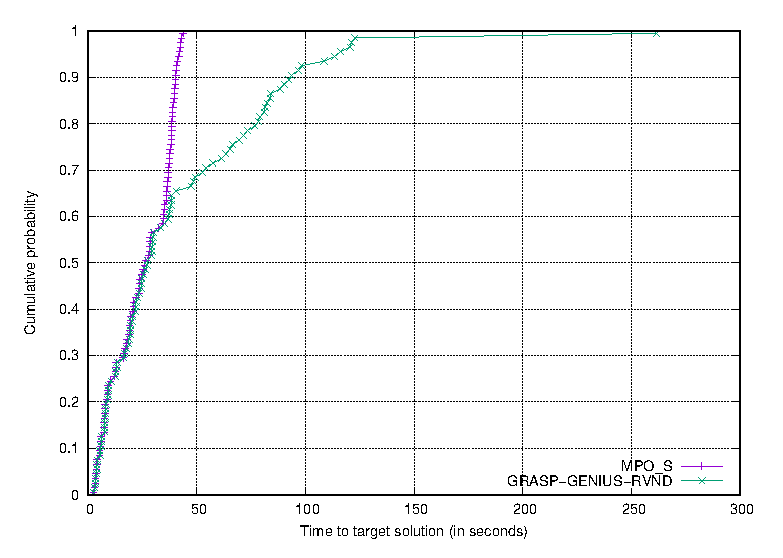
\includegraphics[width=0.5\textwidth]{alvo-12962.eps}
	\caption{TTTplots for kroA150\_R30\_T30\_W90\_50 with 12962 as target}
	\label{fig:tttplots1}%
\end{figure}

\begin{figure}[h]
	\centering
	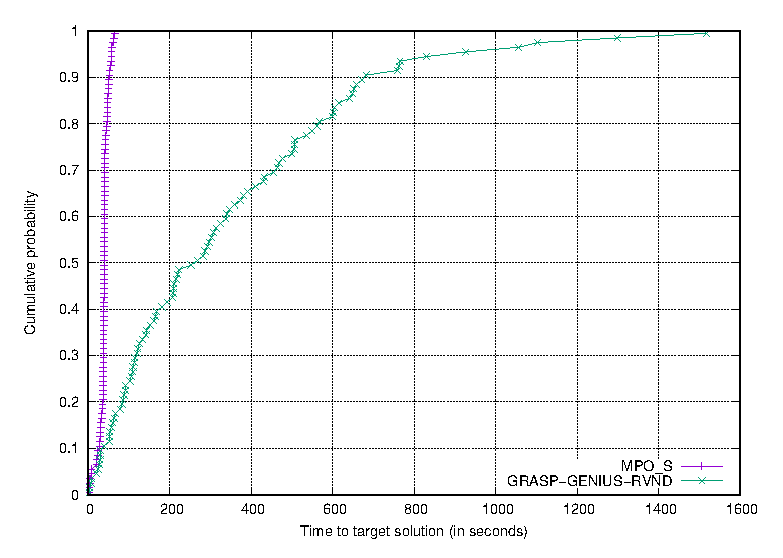
\includegraphics[width=0.5\textwidth]{alvo-12918.eps}
	\caption{TTTplots for kroA150\_R30\_T30\_W90\_50 with 12918 as target}
	\label{fig:tttplots2}%
\end{figure}

In the TTT plots presented in Figures \ref{fig:tttplots1} and \ref{fig:tttplots2}, it is clear the superiority of the proposed hybrid approach concerning the \mbox{GRASP-GENIUS-RVND}, when one determines a target solution value. Looking at the TTT plot for the target 12962 (easy target), shown in Figure \ref{fig:tttplots1}, we can see that the GRASP-GENIUS-RVND indicated a probability of around 66\% to reach the given target in 40 seconds, while MPO\_S presented a probability
of 88\%, of reaching the target within the same time.

For the target 12918 (hard target), illustrated in Figure \ref{fig:tttplots2}, one realises that there is a greater difference in performance between the MPO\_S and GRASP-GENIUS-RVND. After 561 seconds of running time, the state-of-the-art heuristic reaches the target with a probability of 79\%, while with this same probability, the MPO\_S needs only 45.77 seconds, to reach the same target.

\subsection{Statistical analysis}

To strengthen the performance evaluation of the proposed heuristic, statistical significance tests were performed in all the 107 instances. The objective of this test is to verify in statistical terms, if the results obtained by the heuristics indicate a statistical difference, reinforcing the relevance of the application of ILP or not.


Normally, this type of test is used to evaluate algorithms with random components, and to identify whether the difference between their averages solution values was due to the superiority of any of these algorithms, or just due to the randomness present in the methods. In this work, the non-parametric statistical test of Friedman \citep{siegal1956nonparametric} from  R package \citep{r-package} was used, in which it does not require the analysed sample to follow a normal distribution.

In this test, we have set $p$-value equal to 0.05 and two hypotheses:

{\small
\begin{itemize}
\item Null hypothesis ($ H_0 $): There is no difference between the averages values found by the two methods; and

\item Alternative hypothesis ($ H_1 $): There is a difference between the averages values found by the two methods.

\end{itemize}
}

Therefore, $H_0$ will be rejected with 95\% of confidence if, for each instance, Friedman's test returns a value smaller than or equal to the chosen $p$-value. If $H_0$ is rejected, the alternative hypothesis $H_1$ is considered.  Table \ref{tab:sig} presents the number of times the respective heuristic was better in terms of the average solution; and within the parenthesis, the number of results with statistical significance.




\begin{table}[h]
	\centering
	\caption{Analysis of statistical significance}
	\label{tab:sig}
	{\footnotesize
	\begin{tabular}{ll}
		\hline
		Compared strategies & Avg Sol Wins \\
		\hline 

		MPO\_S           & 43(8)        \\
		GRASP-GENIUS-RVND   & 6(0)    \\
		\hline   
	\end{tabular}
}
\end{table}

In terms of the average solution, the MPO\_S outperforms the GRASP-GENIUS-RVND in 43 cases, in which eight are statistically significant. The MPO\_S lost in six cases, and  none of these were statistically significant.


\section{Conclusions}
\label{sec:conclusions}
%- falar pq o GRASP-GENIUS-RNVD eh mais rapido que o MPO

We have approached the PCCTP, a generalisation of the CTP, which is NP-Hard. As exact approaches, we have proposed a new mathematical formulation based on cut-sets constraints, along with a branch-and-cut (B\&C) algorithm; and valid inequalities for improving the linear relaxation of this formulation. 

Following the preprocessing procedures found in the literature, six new reduction rules were proposed, and an investigation was carried out on the best order of their application. As an approximate approach, a new hybrid heuristic has been devised, by combining the state-of-the-art heuristic with ILP (MPO\_S).

The results obtained with the B\&C were far superior to the two formulations in the literature. Considering the one-hour time limit, the proposed B\&C was able to find an optimal solution for most of the instances, and prove unprecedented  optimality for 12 approximate solutions from the literature. An even more satisfactory result was concerning the CPU time spent by exact approaches, in which the B\&C was faster than the best formulation in the literature (Multi-flow) in 97\% of the instances, with an average speedup of 43\%. 


The results of the exact approaches were improved by applying the valid inequalities and the reduction rules. Through an investigation on the best order of its application, the reduction rules increased the number of solved instances in all three formulations. For the proposed B\&C, one realized that, in fact, the proposed inequalities strengthen its linear relaxation, allowing it to reach optimal solutions for 14 more instances. It was not possible to obtain a solid conclusion about the impact of inequalities regarding the CPU-time spent. For some instances, there is an increase in the processing time, and for others, there is a reduction, but when the latter happens it is usually quite significant.

%% AQUI

Considering the results obtained from the heuristics, the MPO\_S  proved to perform better than GRASP-GENIUS-RVND in terms of solution quality and computational time simultaneously, especially for the larger instances. For example, in harder instances (with 202 vertices or more), we observed that the improvements in solution quality made were significant since their numbers of wins over GRASP-GENIUS-RVND were predominant.  Regarding the experiments concerning the CPU-time, when we set a target solution value we observed an even better performance by MPO\_S.


As future investigations, it is intended to develop a new hybrid heuristic, combining data mining and ILP. In this new heuristic, probably a higher quality of the $E^0 $ set would be built, and mined patterns could be used as a warm start for the ILP model. The PCCTP shares structural characteristics with several other problems, then another future work would be to test the robustness of our methods, by adapting them to an application in such problems.


\bibliographystyle{apalike}
\bibliography{bib}

\end{document}
